\documentclass[11pt,letterpaper]{article}
\usepackage[T1]{fontenc}
\usepackage{lmodern,microtype}
\usepackage[margin=1in]{geometry}
\usepackage{amsmath,amssymb,amsthm,mathtools}
\usepackage{booktabs,tabularx,longtable,array,multirow}
\usepackage{xcolor,graphicx}
\usepackage{tikz}
\usetikzlibrary{arrows.meta,positioning,fit,calc,backgrounds,shapes.geometric,shapes.multipart,decorations.pathreplacing}
\usepackage{pgfplots}
\pgfplotsset{compat=1.18}
\usepackage{listings}
\usepackage[numbers,sort&compress]{natbib}
\usepackage{enumitem}
\usepackage{caption}
\usepackage{hyperref}

% Palette: ink/accent for prose and diagrams; two validated data colours
% (blue #2a78d6, orange #eb6834; orange always carries a direct label).
\definecolor{ink}{HTML}{18354A}
\definecolor{accent}{HTML}{126B72}
\definecolor{pale}{HTML}{EEF5F6}
\definecolor{paleink}{HTML}{E4EAF0}
\definecolor{warm}{HTML}{FBEFE6}
\definecolor{muted}{HTML}{52514E}
\definecolor{gridgray}{HTML}{D9D9D6}
\definecolor{seriesA}{HTML}{2A78D6}
\definecolor{seriesB}{HTML}{EB6834}

\hypersetup{colorlinks=true,linkcolor=ink,citecolor=accent,urlcolor=accent,
  pdftitle={Learning, Search and Evidence in a Pokemon Showdown VGC Agent},
  pdfauthor={pokemon-showdown-player project}}
\lstset{basicstyle=\small\ttfamily,breaklines=true,columns=fullflexible,
  frame=single,rulecolor=\color{pale},backgroundcolor=\color{pale},
  showstringspaces=false,keepspaces=true}
\setlist{itemsep=2pt,topsep=5pt}
\setlength{\emergencystretch}{2em}
\captionsetup{font=small,labelfont={bf,color=ink}}

\newtheorem{proposition}{Proposition}[section]
\newtheorem{theorem}[proposition]{Theorem}
\newtheorem{lemma}[proposition]{Lemma}
\newtheorem{definition}[proposition]{Definition}
\newtheorem{example}[proposition]{Example}
\theoremstyle{remark}
\newtheorem{remark}[proposition]{Remark}

\newcommand{\E}{\mathbb{E}}
\newcommand{\Prob}{\mathbb{P}}
\newcommand{\R}{\mathbb{R}}
\newcommand{\A}{\mathcal{A}}
\newcommand{\B}{\mathcal{B}}
\newcommand{\clip}{\operatorname{clip}}
\newcommand{\softmax}{\operatorname{softmax}}
\newcommand{\KL}{D_{\mathrm{KL}}}
\newcommand{\Bin}{\operatorname{Bin}}
\newcommand{\code}[1]{\texttt{\detokenize{#1}}}
\newcommand{\intuition}[1]{\par\smallskip\noindent\textcolor{accent}{\textbf{Interpretation.}} #1\par\smallskip}
\newcommand{\source}[1]{\par\smallskip\begingroup\small\raggedright
  \noindent\textcolor{ink}{\textbf{Implementation:}} #1\par\endgroup\smallskip}
\newcommand{\caveat}[1]{\par\smallskip\noindent\textcolor{seriesB!80!black}{\textbf{Caveat.}} #1\par\smallskip}

% Shared TikZ styles for every diagram.
\tikzset{
  box/.style={draw=ink,rounded corners=3pt,fill=pale,align=center,font=\small,
    minimum height=9mm,inner sep=4pt},
  warmbox/.style={box,fill=warm,draw=seriesB!70!black},
  inkbox/.style={box,fill=paleink},
  note/.style={font=\scriptsize,text=muted,align=center},
  arr/.style={-{Latex[length=2mm]},thick,draw=accent},
  darr/.style={arr,dashed},
  lane/.style={draw=gridgray,fill=white,rounded corners=2pt},
  lanelabel/.style={font=\small\bfseries,text=ink,anchor=east,align=right},
}

\title{\textcolor{ink}{Learning, Search and Evidence in a\\
  Pok\'{e}mon Showdown VGC Agent}\\[0.6em]
  \large Architecture, Data, Training on CPU and Apple~MPS, Decision-Time Search,\\
  and the Mathematics Behind Each Claim}
\author{\texttt{pokemon-showdown-player}\\\small Technical report grounded in the repository implementation}
\date{9 October 2026 (second edition; first edition 7 October 2026)\\
  \small Public source snapshot: \texttt{0c00ec2}; simulator pin \texttt{c046106}; feature schema 1}

\begin{document}
\maketitle
\begin{abstract}
This report describes a complete system for playing the Champions VGC 2026
Regulation~M-C doubles format on Pok\'{e}mon Showdown, and it audits the
mathematics behind each component. Turn decisions are made by a
\emph{determinized simultaneous-move search} run in the official simulator,
over opponent sets sampled from ladder usage statistics. A compact
action-conditioned actor--critic chooses team previews and generates all
training data. A Playwright browser transport clicks the decisions into the
real client. A supervisor schedules three bounded lanes on one Apple~M5
laptop: CPU self-play collection, PPO learning on the Metal (MPS) GPU, and
paired CPU evaluation. A candidate is promoted only after an exact paired sign
test and a set of integrity checks.

We give the exact network, the strategic prior and its temperature, the
per-decision record kept for every match, the PPO loss and its KL stop, the
resource and promotion rules, and the search algorithm. Thirty-one
propositions, theorems and lemmas state their assumptions and are proved.
Eight worked examples recompute the implemented numbers. A new evidence chapter reports the paired
offline result (search 30/45 against the learned policy's 19/45, McNemar
$p=0.0064$), the live record before and after search, and a negative-results
ledger of more than thirty rejected candidates. This edition also corrects the
first: it records stale claims, a circular proposition and an unstated
temperature, and it documents implementation defects found during review.
\end{abstract}

\vspace{0.5em}
\noindent\textbf{Keywords:} Pok\'{e}mon Showdown, VGC doubles, determinization,
regret matching, PPO, action masking, Apple MPS, paired sign test, Elo.

\clearpage
\setcounter{tocdepth}{1}
\tableofcontents
\listoffigures
\clearpage

\section{Introduction and scope}
\label{sec:scope}

The practical question behind this repository is simple to state. Can one
laptop, with no human in the turn loop, play a current VGC format on the
public Showdown ladder, improve from its own experience, and prove each
improvement before relying on it? Answering it takes several kinds of
component, each with its own evidence and failure modes. A transport has to
deliver legal choices on time. A decision procedure has to choose them. A data
recorder has to preserve exactly what was known when each choice was made. A
learner has to turn those records into candidate models. A statistical gate
has to decide which candidates are better. This report explains each
component, gives the mathematics it relies on, and states what has been
measured.

\subsection{What changed since the first edition}
The first edition (7 October 2026) described a persistent MCP harness in
which the OpenClaw agent called tools and a local actor--critic chose every
battle decision. Thirty-three public commits later the deployed system is
different in five ways that matter mathematically:
\begin{enumerate}
  \item \textbf{Turn decisions come from search.} A determinized one-turn
    simultaneous-move search over the official simulator chooses live turn
    actions (Section~\ref{sec:search}). The neural actor now chooses only team
    previews, and it does so greedily.
  \item \textbf{The neural policy has a temperature and a strategic prior.}
    Logits are divided by $\tau=0.25$. The additive prior is no longer the
    legacy power heuristic: it is a squashed one-turn scenario evaluation
    (Sections~\ref{sec:features} and~\ref{sec:network}).
  \item \textbf{Promotion is a hypothesis test.} Candidates must pass an exact
    one-sided paired sign test at $p\le0.05$ as well as a win margin. The worker
    only stages a candidate; promotion happens later at a matchmaking boundary
    (Section~\ref{sec:promotion}).
  \item \textbf{Training is a three-lane pipeline.} CPU collection, PPO on the
    Apple~MPS GPU and CPU evaluation run as separate bounded processes. Each
    trajectory is checked against its collecting likelihood, and PPO stops
    early on a KL criterion (Sections~\ref{sec:learning} and~\ref{sec:pipeline}).
  \item \textbf{Live play is browser-driven.} Playwright clicks the official
    client, guarded by the request identifier. OpenClaw and MCP remain available
    for agent-supervised play but are no longer in the turn loop
    (Section~\ref{sec:transport}).
\end{enumerate}
Appendix~\ref{app:errata} lists every first-edition statement that this
edition corrects, including one circular proposition and several claims made
stale by later commits.

\subsection{Three kinds of statement}
The report keeps three kinds of statement apart:
\begin{enumerate}
  \item \textbf{Implemented behaviour}: facts traceable to source functions,
    such as tensor dimensions, constants and gate predicates. These are
    followed by an \emph{Implementation} line naming the files.
  \item \textbf{Conditional mathematical results}: propositions proved under
    explicit assumptions, followed by an \emph{Interpretation} or
    \emph{Caveat} that says how far the result transfers to the running system.
  \item \textbf{Measurements}: results of experiments run by the project,
    cited to the repository's validation documents or, where marked, to the
    local run ledger. This paper ran no new games, training or promotion, apart
    from read-only recomputation of the statistics it reports.
\end{enumerate}

\subsection{Format and pinned mechanics}
The main target is \code{gen9championsvgc2026regmc}: doubles, bring six and
pick four, open team sheets on request, one Mega Evolution per battle, no
Terastallization, Item and Species Clauses, and Champions stat points instead
of EVs and IVs \citep{championsrules}. The local simulator dependency is
pinned to official Showdown commit
\code{c046106cbe075931b1ff8d8b800ff5be47a85f96} \citep{showdownsource}. A
format identifier beginning with \code{gen9} does not determine these
mechanics. Format, simulator revision, feature profile, team fingerprint and
collecting checkpoint are part of every scientific statement in this report.

\subsection{Summary of measured results}
\begin{table}[htbp]
\centering\small
\begin{tabularx}{\linewidth}{>{\raggedright\arraybackslash}p{0.34\linewidth} X}
\toprule
Question & Measured answer (details in Section~\ref{sec:evidence}) \\
\midrule
Does search beat the learned policy offline? & Same 45 seeds, sides and real
opponent teams: search 30/45 vs.\ policy 19/45; 14 gains, 3 losses; exact
McNemar $p=0.0064$. Clustering by opponent team: $p=0.0037$. \\
Did the learned policy improve over campaigns? & Live record 348--499 (41.1\%)
over 847 games across three actor generations. One strategic prior passed an
independent 160-game final (125 vs.\ 106, $p=0.0072$). One PPO update passed
the 60-game gate out of 129 attempts. \\
What happened live after search? & Preliminary and observational: 41 games,
27--14. Rating 1182 $\rightarrow$ 1464. Elo-expected 18.4 wins in 37 rated
games; observed 23 (exact $p=0.086$). \\
What failed? & More than thirty candidates: PPO variants, preview models, a
matchup architecture that passed development and then tied its final, and an
offline hyperparameter matrix with no significant arm after Holm correction. \\
\bottomrule
\end{tabularx}
\caption{Headline evidence. Ladder results depend on the opponent pool and on
rating-based matchmaking; Section~\ref{sec:elo} explains why a raw win rate is
not a stable strength measure.}
\label{tab:headline}
\end{table}

\subsection{How to read this report}
Section~\ref{sec:system} gives the system map and project timeline.
Sections~\ref{sec:game}--\ref{sec:network} formalize the game, the candidate
actions, the features and the neural policy. Section~\ref{sec:data} describes
the record kept for every match. Sections~\ref{sec:learning}--\ref{sec:promotion}
cover learning, the CPU/MPS pipeline and promotion statistics.
Section~\ref{sec:search} analyses the search agent and
Section~\ref{sec:transport} the live turn. Section~\ref{sec:scout} covers
opponent-move scouting and team selection. Section~\ref{sec:evidence} collects
all evidence and Section~\ref{sec:limits} its limits. The appendices provide a
glossary, the corrections to the first edition, defects found during review, a
source map and reproduction notes.

\section{System overview}
\label{sec:system}

\subsection{Components and responsibilities}
Figure~\ref{fig:architecture} shows the deployed system. It has three
columns. The \emph{play} column talks to Showdown. The \emph{decide} column
chooses actions. The \emph{learn} column turns recorded games into candidate
models and decides whether to deploy them. The arrows that cross columns are
narrow on purpose. A decision procedure receives a context built from public
information and the player's own request, and returns one complete choice
string. A learner receives completed, validated records and returns a
checkpoint file. Deployment is one atomic file replacement made at a
matchmaking boundary.

\begin{figure}[htbp]
\centering
\resizebox{\linewidth}{!}{%
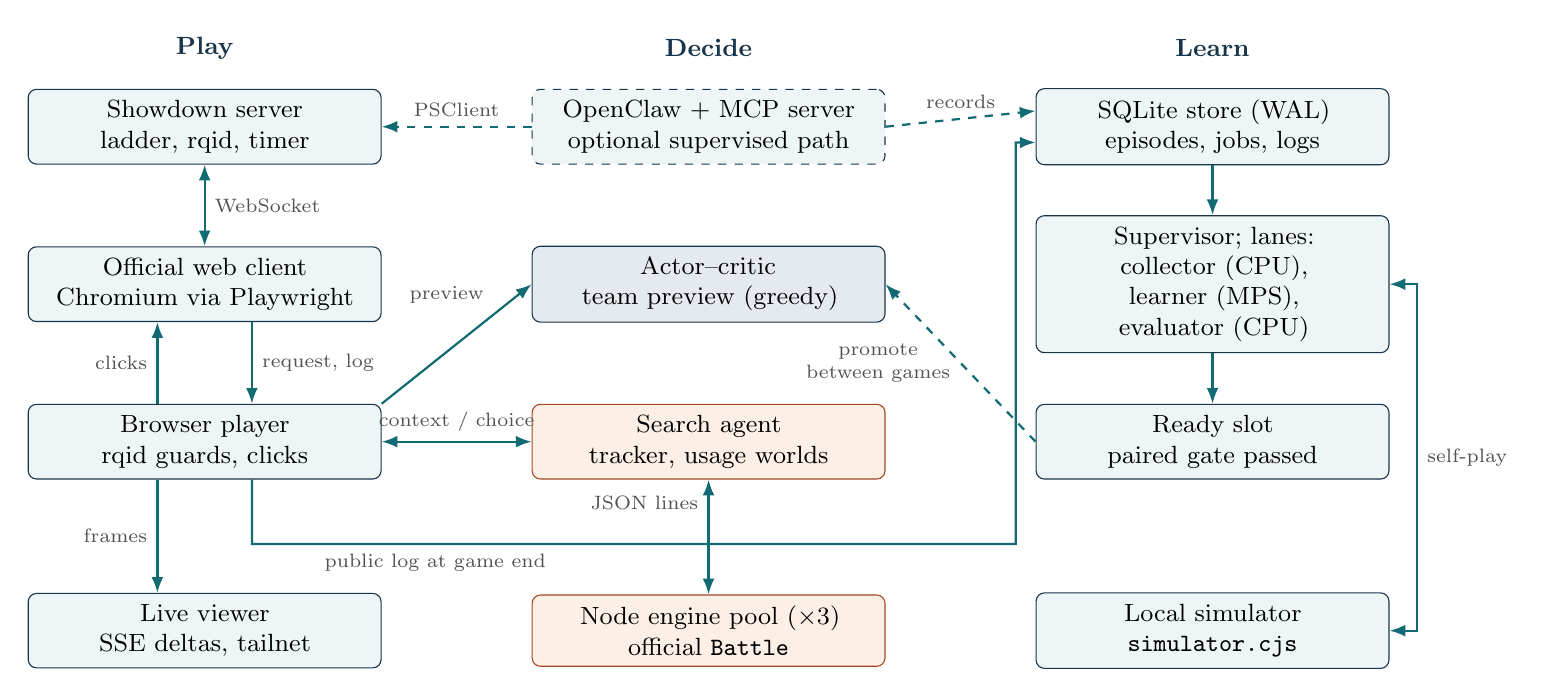
\begin{tikzpicture}[x=1cm,y=1cm]
  \tikzset{col/.style={box,text width=42mm}}
  \node[font=\small\bfseries,text=ink] at (0,1.0) {Play};
  \node[font=\small\bfseries,text=ink] at (6.4,1.0) {Decide};
  \node[font=\small\bfseries,text=ink] at (12.8,1.0) {Learn};
  \node[col] (server) at (0,0) {Showdown server\\ladder, rqid, timer};
  \node[col] (client) at (0,-2) {Official web client\\Chromium via Playwright};
  \node[col] (player) at (0,-4) {Browser player\\rqid guards, clicks};
  \node[col] (viewer) at (0,-6.4) {Live viewer\\SSE deltas, tailnet};
  \node[col,dashed] (mcp) at (6.4,0) {OpenClaw + MCP server\\optional supervised path};
  \node[col,fill=paleink] (actor) at (6.4,-2) {Actor--critic\\team preview (greedy)};
  \node[col,fill=warm,draw=seriesB!70!black] (search) at (6.4,-4) {Search agent\\tracker, usage worlds};
  \node[col,fill=warm,draw=seriesB!70!black] (engines) at (6.4,-6.4) {Node engine pool ($\times3$)\\official \code{Battle}};
  \node[col] (store) at (12.8,0) {SQLite store (WAL)\\episodes, jobs, logs};
  \node[col] (lanes) at (12.8,-2) {Supervisor; lanes:\\collector (CPU), learner (MPS),\\evaluator (CPU)};
  \node[col] (ready) at (12.8,-4) {Ready slot\\paired gate passed};
  \node[col] (sim) at (12.8,-6.4) {Local simulator\\\code{simulator.cjs}};
  \draw[arr,{Latex[length=2mm]}-{Latex[length=2mm]}] (server) -- node[note,right]{WebSocket} (client);
  \draw[arr] ([xshift=6mm]client.south) -- node[note,right]{request, log} ([xshift=6mm]player.north);
  \draw[arr] ([xshift=-6mm]player.north) -- node[note,left]{clicks} ([xshift=-6mm]client.south);
  \draw[arr] ([xshift=-6mm]player.south) -- node[note,left]{frames} ([xshift=-6mm]viewer.north);
  \draw[arr,{Latex[length=2mm]}-{Latex[length=2mm]}] (player) -- node[note,above]{context / choice} (search);
  \draw[arr] (player.north east) -- node[note,above left,pos=.75]{preview} (actor.west);
  \draw[arr,{Latex[length=2mm]}-{Latex[length=2mm]}] (search) -- node[note,left,pos=.2]{JSON lines} (engines);
  \draw[arr] ([xshift=6mm]player.south) |- node[note,below,pos=.62]{public log at game end} (10.3,-5.3)
     -- (10.3,-0.2) -- ([yshift=-2mm]store.west);
  \draw[darr] (mcp.west) -- node[note,above]{PSClient} (server.east);
  \draw[darr] (mcp.east) -- node[note,above]{records} ([yshift=2mm]store.west);
  \draw[arr] (store) -- (lanes);
  \draw[arr] (lanes) -- (ready);
  \draw[arr,{Latex[length=2mm]}-{Latex[length=2mm]}] (lanes.east) -- ++(0.35,0) |- node[note,right,pos=.25]{self-play} (sim.east);
  \draw[darr] (ready.west) -- node[note,left,pos=.5,align=center]{promote\\between games} (actor.east);
\end{tikzpicture}}
\caption{Deployed responsibilities on 9 October 2026. Orange boxes are the
decision-time search. The learned actor chooses only the team preview live,
but it generates all training data in self-play. The dashed promotion path
replaces the actor between games, after a candidate has passed the paired gate
and integrity checks. The dashed MCP path supports agent-supervised play and
recording; it is not used by the browser runner.}
\label{fig:architecture}
\end{figure}

\subsection{Processes, devices and cadence}
\begin{table}[htbp]
\centering\small
\begin{tabularx}{\linewidth}{>{\raggedright\arraybackslash}p{0.2\linewidth}
  >{\raggedright\arraybackslash}p{0.13\linewidth} X}
\toprule
Process & Device & Role and cadence \\
\midrule
Browser runner & CPU & One account lock. Plays ladder games through the
official client, with a 30-second gap between games. Calls promotion before
each matchmaking search. \\
Search engines & CPU (3 Node) & Long-lived simulator processes. Each turn they
receive 2 of the 6 sampled worlds; median decision 2.3\,s. \\
Supervisor & CPU & launchd \code{KeepAlive}. Polls every 15\,s, samples host
resources, and runs at most one child per lane. \\
Collector lane & CPU & Self-play in spawned one-thread processes, each driving
a Node simulator. Writes complete sampled episodes. \\
Learner lane & MPS GPU & PPO on validated episodes; at most 12\% of recommended
Metal memory; falls back to CPU on device errors. Then a scout update. \\
Evaluator lane & CPU & Paired incumbent and candidate panels with frozen
inputs; the exact sign-test gate; staging. \\
Live viewer & CPU & Publishes filtered public frames every 0.2\,s over SSE. \\
Cold archiver & CPU & Every 900\,s, gzip-archives completed inference inputs
with SHA-256 verification. \\
\bottomrule
\end{tabularx}
\caption{Long-running processes on the always-on Apple~M5 host (10 cores,
16\,GB unified memory). The lanes are described in Section~\ref{sec:pipeline}.}
\label{tab:processes}
\end{table}

\subsection{Project timeline}
Figure~\ref{fig:timeline} places the changes analysed in this report in
time. The dates explain an important feature of the evidence. The 847-game
live record spans three actor generations and two transports, so it is not
a measurement of any single policy.

\begin{figure}[htbp]
\centering
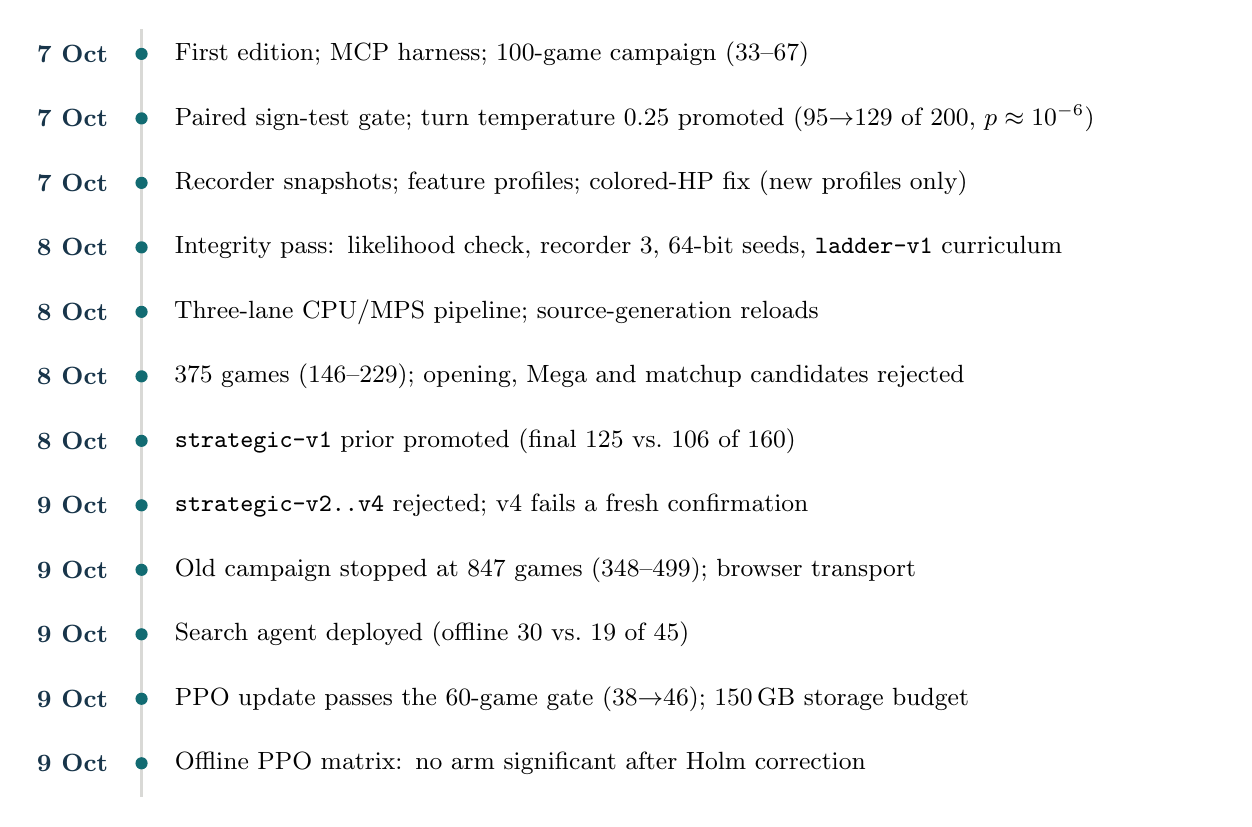
\begin{tikzpicture}[x=1cm,y=0.78cm]
  \draw[very thick,draw=gridgray] (0,0.4) -- (0,-12.1);
  \foreach \y/\d/\t in {
    0/{7 Oct}/{First edition; MCP harness; 100-game campaign (33--67)},
    -1.05/{7 Oct}/{Paired sign-test gate; turn temperature 0.25 promoted (95$\to$129 of 200, $p\approx10^{-6}$)},
    -2.1/{7 Oct}/{Recorder snapshots; feature profiles; colored-HP fix (new profiles only)},
    -3.15/{8 Oct}/{Integrity pass: likelihood check, recorder~3, 64-bit seeds, \code{ladder-v1} curriculum},
    -4.2/{8 Oct}/{Three-lane CPU/MPS pipeline; source-generation reloads},
    -5.25/{8 Oct}/{375 games (146--229); opening, Mega and matchup candidates rejected},
    -6.3/{8 Oct}/{\code{strategic-v1} prior promoted (final 125 vs.\ 106 of 160)},
    -7.35/{9 Oct}/{\code{strategic-v2..v4} rejected; v4 fails a fresh confirmation},
    -8.4/{9 Oct}/{Old campaign stopped at 847 games (348--499); browser transport},
    -9.45/{9 Oct}/{Search agent deployed (offline 30 vs.\ 19 of 45)},
    -10.5/{9 Oct}/{PPO update passes the 60-game gate (38$\to$46); 150\,GB storage budget},
    -11.55/{9 Oct}/{Offline PPO matrix: no arm significant after Holm correction}}
  {
    \fill[accent] (0,\y) circle (2.2pt);
    \node[anchor=east,font=\small\bfseries,text=ink] at (-0.3,\y) {\d};
    \node[anchor=west,font=\small,text width=13.2cm] at (0.3,\y) {\t};
  }
\end{tikzpicture}
\caption{Chronology of the public commits from \code{153e3db} to
\code{0c00ec2} (7--9 October 2026). The results are recomputed in
Section~\ref{sec:evidence}.}
\label{fig:timeline}
\end{figure}

\subsection{Two transports, one decision contract}
The repository keeps two ways to reach Showdown. Both obey the same contract:
a decision is one complete choice string for one actionable request, and it is
taken from the request-visible candidate list $\A(r)$ of
Section~\ref{sec:actions}.
\begin{itemize}
  \item \textbf{MCP harness.} \code{ps_mcp_server.py} registers 41 tools.
    The groups are connection, teams, play, model, learning and research. A
    single \code{PSClient} WebSocket logs in with a challenge-string
    assertion and sends \code{ROOMID|/choose CHOICE}
    \citep{mcptools,mcptransport,showdownprotocol}. OpenClaw's native registry
    exposes the tools as \code{pokemonshowdown__ps_*}. A retained session keeps
    the server process across turns; a detached one-shot run retires it
    \citep{openclawregistry}. This path still records decisions and can resume
    one pending episode after a disconnect.
  \item \textbf{Browser runner.} \code{scripts/browser_play.py} drives the
    official client with Playwright. It reads \code{app.rooms[id]} and clicks
    visible controls. Decisions come from local inference or search; no
    language model is in the turn loop (Section~\ref{sec:transport}).
\end{itemize}
The two paths have different recording rules. MCP play can record sampled PPO
data. A browser game played with \code{--search} is never a PPO sample,
because its actions do not come from the actor's distribution. It contributes
only its public log to the scout corpus (Section~\ref{sec:scout}).

\source{\code{ps_mcp_server.py}, \code{ps_client.py}, \code{harness.py},
\code{ml/live.py}, \code{ml/browser.py}, \code{scripts/browser_play.py},
\code{scripts/browser_service.py}, \code{scripts/learning_service.py}.}

\section{The battle as a partially observed stochastic game}
\label{sec:game}

\subsection{State, actions and observations}
Let $s_t$ be the complete battle state at a decision boundary. It includes
both teams' hidden sets, current HP, statuses, field conditions, pending
mechanics and the simulator's random-number state. Player~1 chooses a complete
action $a_t$ and player~2 chooses $b_t$ simultaneously. Chance $\xi_t$ affects
the transition:
\begin{equation}
  s_{t+1}\sim P(\cdot\mid s_t,a_t,b_t),\qquad
  o^i_{t+1}\sim O_i(\cdot\mid s_{t+1}),\quad i\in\{1,2\}.
  \label{eq:posg}
\end{equation}
A real trace also contains team preview, forced replacements and waiting
requests. In the learner, the index $t$ counts \emph{recorded actionable
requests}, not battle turns. Holding the opponent's strategy fixed reduces the
game to a single-agent partially observed control process. If the opponent's
behaviour depends on its own history, that history must be part of the latent
state.

Write $h_t$ for the information available to our player before decision $t$:
the public protocol prefix, our own private requests and our past actions. An
exact Bayesian belief is $\beta_t(s)=\Prob(s_t=s\mid h_t)$. For a fixed
opponent with joint kernel $\bar P$ and observation kernel $O$, it updates by
\begin{equation}
  \beta_{t+1}(s')
  =\frac{O(o_{t+1}\mid s')\sum_s\bar P(s'\mid s,a_t)\beta_t(s)}
  {\sum_u O(o_{t+1}\mid u)\sum_s\bar P(u\mid s,a_t)\beta_t(s)},
\label{eq:belief}
\end{equation}
whenever the denominator is positive \citep{kaelbling,smallwood1973}. Nothing
in the repository computes Equation~\eqref{eq:belief}. The neural policy
compresses $h_t$ into a feature vector $x_t=\phi(h_t)$
(Section~\ref{sec:features}). The search agent replaces the belief with a
\emph{sampling distribution} over opposing sets, built from ladder usage
statistics and conditioned on what has been revealed
(Section~\ref{sec:search}). Both are approximations to $\beta_t$, and neither
is calibrated.

\subsection{What the format reveals}
Champions M-C makes some hidden information public. Team preview reveals all
six opposing species. When open team sheets are exchanged, the opposing
species, items, abilities, moves and natures become known. Stat-point
allocations stay hidden, and IVs are unused in this format. The audit in
\code{docs/match-data-collection.md} found this pattern directly. Over 50
audited games, our own nature and stat points were stored in all 50. The
opponent's nature was disclosed in 2, and its stat points in none. Open sheets
are therefore informative but not complete. Only the damage-relevant stat
spread remains latent once sheets are shown, but that spread alone moves
damage rolls across KO thresholds.

\intuition{An opposing Pok\'{e}mon at 50\% HP is an observation. Its
unrevealed item is a latent variable. A predicted Protect is a learned
forecast. A sampled stat spread is one hypothesis drawn from a population
model. None of these is a recovered hidden state.}

\subsection{Non-anticipation}
Both decision procedures read only the request and the public prefix. This
can be stated precisely.

\begin{proposition}[Conditional non-anticipation]
\label{prop:information}
Fix the auxiliary inputs: the encoder and its feature profile, the cached dex,
the checkpoint (including its embedded \code{strategy_knowledge}), the frozen
research and scout snapshots, our own team sets and, for search, the usage
table and random seed. Suppose the request and protocol prefix supplied at
decision $t$ contain only information available to our player by $t$. Then
the neural features and the search agent's sampled worlds are measurable
functions of $h_t$ and those inputs. Two calls with the same request, prefix
and inputs produce the same features, and the same distribution over sampled
worlds, whatever happens later and whatever remains unrevealed.
\end{proposition}
\begin{proof}
\code{observe} and \code{Tracker.feed} scan only the supplied prefix and merge
only the supplied own request. Neither queries the opponent's private stream
or any later log suffix. Feature construction is deterministic in the
observation, the candidate string and the fixed inputs. The scout is a fixed
function of a filtered public prefix. The search agent samples worlds from a
distribution that depends on the tracker state, the usage table and the seed.
Composition of measurable maps proves the claim.
\end{proof}

The premise matters. Passing an omniscient log to \code{observe} would
invalidate it. The local simulator bridge therefore observes through the
separate \code{getPlayerStreams().p1/p2} streams; its omniscient stream only
drives the simulator \citep{simprotocol,battlestream}. The proposition also
does not certify an experiment's chronology. The checkpoint's
\code{strategy_knowledge} and the scout are trained on earlier games, and a
held-out evaluation must not include games those earlier models were fitted
on.

\caveat{Inside each sampled world the search engine is \emph{omniscient}
about that world. Both players' sets are fixed and known to both simulated
sides. Non-anticipation holds for the world-sampling step. The per-world
matrix game, however, is a perfect-information model of an imperfect-information
game. Section~\ref{sec:fusion} analyses the bias this introduces.}

\subsection{How faithful the observation is}
The parser covers a selected subset of protocol events. Missing condition data
maps to full HP. Under the deployed \code{strategic-v1} profile, the state
encoder still uses the \emph{legacy} HP parser. A coloured public HP string
such as \code{50/100y} fails to parse and becomes 1.0. The bug was fixed only
for the \code{tactics-v1}, \code{rain-v1} and \code{opening-v1} profiles. In
the last 60 ladder games, 16 of 2{,}509 opposing condition entries carried a
colour suffix, affecting 8 of 523 decisions. The strategic prior itself uses
the corrected parser, so the defect reaches the network's learned residual
but not its prior. Historical observed opponent moves are stored as
\code{moves_known} and used by the planner; \code{Features._mon} encodes
\code{moves}. Perspective correctness therefore does not imply a sufficient
representation.

\source{\code{observe}, \code{hp_fraction} and \code{legacy_hp_fraction} in
\code{battle_state.py}; \code{Features} in \code{ml/features.py};
\code{search/tracker.py}; \code{simulator.cjs}.}

\section{Candidate actions and doubles constraints}
\label{sec:actions}

\subsection{Actions are complete player decisions}
For an actionable request $r$, let $\A(r)$ be the list returned by
\code{legal_choices(r)}. In doubles, one candidate is a complete pair
$a=(u_1,u_2)$. Each $u_i$ is a move slot with a target, a switch destination
or a pass. Examples are
\begin{lstlisting}
move 1 1, move 2 -1
move 1 2 mega, switch 4
\end{lstlisting}
Positive targets are opposing positions and negative targets are our own. The
opponent's simultaneous choice is \emph{not} part of a candidate. The
enumerator takes the Cartesian product of the per-position options. It
removes combinations that violate shared constraints, filters disabled or
exhausted moves, respects visible trapping, and handles fainted positions.
More than two active positions are rejected. Hidden restrictions can still
make the server refuse a candidate, so $\A(r)$ is \emph{request-visible
admissibility}, not proof of acceptance.

\begin{proposition}[Constraints enforced by joint enumeration]
\label{prop:joint}
Every emitted doubles candidate has distinct switch destinations, at most one
Mega-family activation and at most one Terastallization. In a
forced-replacement request, the number of switching positions equals
$\min(\text{forced positions},\text{available bench members})$.
\end{proposition}
\begin{proof}
Each product element is tested in turn. Its switch strings must form a set,
so duplicates are rejected. Under forced switching, its switch count must
equal the stated minimum. Elements with more than one Mega-family event or
more than one Terastallization event are rejected. An emitted element has
passed every predicate.
\end{proof}

The proposition covers these predicates only. Champions requests never offer
Terastallization, so that branch is dormant. Team validation and other hidden
mechanics are outside its scope.

\subsection{Team preview and an exact symmetry}
With $n$ party members and $k$ to bring, preview candidates are ordered
selections, $|\A_{\mathrm{preview}}|=n!/(n-k)!$, which is 360 for six choose
four. The first two positions lead; the last two are the bench. Under
\code{opening-v2} and every \code{strategic-*} profile except
\code{strategic-turn-v1}, the action encoder
canonicalizes the bench by sorting its indices before hashing. The
representation is therefore exactly invariant to swapping the two bench
positions. The actor still scores all 360 candidates, so each plan appears
twice.

\begin{proposition}[Bench symmetry halves the preview space]
\label{prop:preview}
Let $\sim$ identify two preview candidates that agree in their ordered leads
and in their bench as a set. For six choose four this gives 180 classes of
exactly two candidates each. If the features, and hence the logits, are
constant on each class, then:
\begin{enumerate}
  \item the class probabilities $\Pi(C)=\sum_{a\in C}\pi(a)$ are a softmax
    over the 180 class logits, at the same temperature;
  \item the PPO ratio of any candidate equals the ratio of its class;
  \item the candidate-level entropy is $H(\pi)=H(\Pi)+\log2$.
\end{enumerate}
\end{proposition}
\begin{proof}
There are $6\cdot5=30$ ordered lead pairs. Each leaves four members, from
which $\binom{4}{2}=6$ bench sets can be formed, so there are 180 classes.
Each bench set has exactly two orderings, which accounts for all
$180\cdot2=360$ candidates. Let $\ell_C$ be the shared logit. Then
$\pi(a)=e^{\ell_C/\tau}/\sum_{C'}2e^{\ell_{C'}/\tau}$ for $a\in C$, so
$\Pi(C)=2\pi(a)=e^{\ell_C/\tau}/\sum_{C'}e^{\ell_{C'}/\tau}$. The ratio
$\pi_\theta(a)/\pi_{\mathrm{old}}(a)=\Pi_\theta(C)/\Pi_{\mathrm{old}}(C)$
because the factor~2 cancels. Finally,
$H(\pi)=-\sum_C2\pi_C\log\pi_C=-\sum_C\Pi(C)\log(\Pi(C)/2)=H(\Pi)+\log2$.
\end{proof}

\intuition{The duplication is harmless for learning. Ratios are unchanged, and
the entropy bonus is shifted by a constant whose gradient is zero. Statements
such as ``the policy chooses among 360 previews'' should still say 180 distinct
plans. Lead order is kept on purpose: it fixes which Pok\'{e}mon occupies the
left and right positions.}

\subsection{Why joint scoring rather than a product policy}
Sampling each position independently gives
$\pi(u_1,u_2\mid x)=p(u_1\mid x)q(u_2\mid x)$. That family cannot express
coordination.

\begin{proposition}[A coordination a product policy cannot represent]
\label{prop:product}
With two options $A,B$ per position, no unmasked product distribution gives
positive mass to both $(A,A)$ and $(B,B)$ and zero mass to both $(A,B)$ and
$(B,A)$.
\end{proposition}
\begin{proof}
Positive diagonal mass forces $p(A),q(A),p(B),q(B)>0$, so the off-diagonal
products are positive too. Equivalently, every product table has rank one and
determinant zero. The required table has determinant
$\pi(A,A)\pi(B,B)>0$.
\end{proof}

The implemented alternative scores each feasible complete candidate directly.
Masking a product policy with joint constraints, or factorizing it
autoregressively, would also introduce dependence. Feature collisions and
finite capacity still limit which joint distributions the network can express.

\subsection{Two enumerators}
The search engine enumerates candidates separately, inside the simulator, in
\code{sideChoices} of \code{search/engine.cjs}. Its pruning differs from
$\A(r)$:
\begin{itemize}
  \item Damaging moves aimed at the partner are removed.
  \item Targets in empty foe slots are removed while the other foe is alive.
  \item Every move of a Mega-capable Pok\'{e}mon carries the \code{mega} flag,
    so delaying Mega Evolution is never considered.
\end{itemize}
Our own live choices still start from $\A(r)$ and are pruned in Python. The
engine enumeration is used for the opponent and for our forced-replacement
look-ahead. Appendix~\ref{app:defects} records a defect in it: when both
actives on one side can Mega Evolve, every move-and-move pair is discarded.

\source{\code{legal_choices} in \code{battle_state.py}; bench canonicalization
in \code{Features.action} (\code{ml/features.py}); \code{_prune_ours} in
\code{search/agent.py}; \code{sideChoices} in \code{search/engine.cjs}.}

\section{Features, profiles and the strategic prior}
\label{sec:features}

\subsection{Fixed-dimensional vectors for variable objects}
The state vector has $d_s=384$ coordinates and each candidate's action vector
has $d_a=192$. A named feature $f$ with value $v_f$ is added by signed hashing:
\begin{equation}
  \phi_j \mathrel{+}=\sigma(f)\,v_f,\qquad
  j=H(f)\bmod(d-16),\qquad \sigma(f)\in\{-1,+1\}.
\end{equation}
Both $H$ and $\sigma$ come from an eight-byte BLAKE2b digest: the first four
bytes, little-endian, give $H$, and the parity of the fifth byte gives the
sign. The last sixteen coordinates are reserved for dense numbers. That
leaves 368 hashed state buckets and 176 hashed action buckets. Feature names
are namespaced by role and position: species, item, ability, HP, status,
boosts, stats, types, moves with their PP ratio, volatiles, field and side
conditions. The last sixteen public move events are added with weight
$1/\sqrt{i+1}$, counting back from the newest. A research prior adds
\code{meta/<species>} frequencies. It is built from the top 32 team-sheet
frequencies, overlaid by the top 32 usage entries. Dense state slots hold turn
progress $\min(\text{turn}/50,2)$, total own HP divided by six, and
$|\A|/1000$.

The whole vector is clipped to $[-5,5]$. After clipping, the decision code
adds the scout's top-three move probabilities
(Section~\ref{sec:scout}). The \emph{stored} state therefore can leave the
clipped interval.

\begin{proposition}[Hashing loses distinctions]
\label{prop:hash}
A signed hash map from $m$ categorical indicator coordinates into $d'<m$
buckets ($d'=d-16$ here) is not injective on $\R^m$. Any later function of the
hashed vector, including clipping, cannot restore the lost distinctions.
\end{proposition}
\begin{proof}
The map is linear with rank at most $d'<m$, so its null space is nontrivial.
Two inputs that differ by a null-space vector hash to the same output, and
any later function maps equal inputs to equal outputs.
\end{proof}
This is a capacity statement, not a claim that two particular battle states
collide. Expected-collision results for feature hashing assume random hash
functions \citep{featurehashing}; a fixed digest over a realized vocabulary
does not inherit them automatically.

\subsection{Feature profiles}
A checkpoint stores a \code{feature_profile}. Training excludes episodes
recorded under any other profile, so a profile is a versioned input semantics.
The schema number alone is not enough to identify the inputs. Nineteen profiles
exist; Table~\ref{tab:profiles} lists the families.

\begin{table}[htbp]
\centering\small
\begin{tabularx}{\linewidth}{>{\raggedright\arraybackslash}p{0.27\linewidth} X}
\toprule
Profile family & What it changes \\
\midrule
\code{legacy}, \code{weather-v1} & Original features and the power/type prior
of Section~\ref{sec:legacyprior}; weather-aware move data. \\
\code{tactics-v1}, \code{rain-v1}, \code{mechanics-v1} & Damage-based turn
priors and rain-team mechanics. \code{tactics-v1} and \code{rain-v1}, with
\code{opening-v1}, are the only profiles that use the corrected coloured-HP
parser. \\
\code{preview-*}, \code{lineup-v1}, \code{opening-*}, \code{mega-v1} &
Preview priors (coverage, lead pressure, exposure) and exact prospective Mega
stats under Champions rules. \\
\code{strategic-v1} (\textbf{deployed}) & Scenario-evaluation prior for turns
and previews (Section~\ref{sec:strategic}); bench canonicalization. \\
\code{strategic-v2..v5} & More mechanics, preview plan summaries, Mega
uncertainty. v2--v4 were evaluated and rejected; the v5 experiment was paused
before a completed gate (Section~\ref{sec:evidence}). \\
\bottomrule
\end{tabularx}
\caption{Feature-profile families. Only \code{strategic-v1} is deployed.}
\label{tab:profiles}
\end{table}

\subsection{The deployed strategic prior}
\label{sec:strategic}
The final action coordinate holds a scalar prior $q_0(x,a)$. Under
\code{strategic-v1} it comes from a one-turn \emph{scenario evaluation} in
\code{ml/strategy.py}, which has four steps.

\paragraph{Opponent hypotheses.}
For each live opposing active Pok\'{e}mon, candidate moves are drawn from the
disclosed sheet if there is one. Otherwise they are the observed moves plus
the five most frequent executed moves for the species in the checkpoint's
\code{strategy_knowledge}. That table holds counts from 766 earlier games.
Each move gets the weight
\begin{equation}
  w=2+\sqrt{\text{count}}+\min(3,\text{recent}),
\end{equation}
with Protect multiplied by 1.5 below 40\% HP, by 0.65 otherwise, and by 0.3
if it was used on the previous turn. The two strongest attacks and one support
move are kept. A single-target attack is split over targets: weight~1 goes to
the target with the largest damage relative to its remaining HP
($\text{damage}/\max(0.2,h)$), and 0.45 to the others. Two further hypotheses are
added when they apply:
\begin{itemize}
  \item a switch-in from the revealed bench, with weight $0.12\sum w$;
  \item a 50/50 Mega-forme split, when the stone is disclosed and the side's
    Mega is unspent.
\end{itemize}

\paragraph{Joint scenarios.}
Per-position hypotheses are multiplied across the two opposing positions.
Impossible combinations, such as two Megas or two switches into one reserve,
are removed. The six most probable scenarios are kept and renormalized to
probabilities $p_k$.

\paragraph{Deterministic resolution.}
For our candidate $a$ and scenario $k$, \code{simulate} resolves one turn in
priority and speed order, including Trick Room. It accounts for Protect, Wide
Guard, redirection, Helping Hand, Fake Out, weather, terrain, Intimidate on
entry, drain, recoil and Focus Sash. Damage uses the standard formula
\begin{equation}
  \text{dmg}=\Big(\tfrac{22\,\mathrm{BP}\,A/D}{50}+2\Big)\cdot\mathrm{STAB}\cdot E\cdot
  \text{burn}\cdot\text{weather}\cdot0.75^{[\text{spread}]}\cdot0.925\cdot\text{acc}\,/\,\text{maxHP},
\end{equation}
where unknown stats are approximated as base~$+\,35$ with stage multipliers, and
unknown maximum HP as base HP~$+\,90$. The constant 0.925 is the mean damage
roll. The outcome value is
\begin{equation}
  v_k(a)=\sum_{\text{foes}}\big[\Delta h+0.8\,\mathbf 1_{\mathrm{KO}}\big]
  -\sum_{\text{own}}\big[\Delta h(1+0.2\rho)+(0.9+\rho)\mathbf 1_{\mathrm{KO}}\big]
  -0.08\,\#\text{Protect}-0.10\,\#\text{switch}+\dots,
\end{equation}
where $\rho\in[0,0.5]$ is a scarcity bonus for a Pok\'{e}mon that is the only
good answer to some opponent. Smaller terms reward a switch-in's next-turn
threat and penalize spending the Mega.

\paragraph{Risk-sensitive aggregation and squashing.}
If speeds tie, each $v_k$ averages both orders. The turn score is
\begin{equation}
  s(a)=3\Big[(1-\kappa)\sum_kp_kv_k(a)+\kappa\min_kv_k(a)\Big],\qquad
  \kappa=\clip\big(0.15+0.05(R_{\mathrm{own}}-R_{\mathrm{foe}}),0.05,0.25\big),
  \label{eq:turnscore}
\end{equation}
where $R_{\mathrm{own}}$ sums our HP fractions. $R_{\mathrm{foe}}$ sums the
revealed foes' HP fractions and counts each unseen foe as one. Preview
candidates use \code{opening_score} instead. It takes the better of no-Mega
and one-Mega modes over coverage, lead pressure and exposure, adds terms for
rain dependency, Intimidate, Fake Out and Trick Room, and doubles the total.
Finally,
\begin{equation}
  q_0(a)=g(s(a)),\qquad g(s)=\frac{4s}{4+|s|}.
  \label{eq:squash}
\end{equation}

\begin{proposition}[Properties of the risk aggregate and the squash]
\label{prop:squash}
\leavevmode
\begin{enumerate}
  \item For any scenario values,
    $\min_kv_k\le(1-\kappa)\sum_kp_kv_k+\kappa\min_kv_k\le\sum_kp_kv_k$.
    The aggregate is monotone in each $v_k$, and adding a constant $c$ to every
    $v_k$ adds $c$ to it.
  \item The function $g$ is odd, strictly increasing and a bijection from $\R$
    onto $(-4,4)$. It satisfies $0<g'(s)=16/(4+|s|)^2\le1$, so it is
    1-Lipschitz. Its ranking of candidates equals the ranking by $s$.
\end{enumerate}
\end{proposition}
\begin{proof}
(1) Since $\min_kv_k\le\sum_kp_kv_k$, a convex combination of the two lies
between them. Each part is monotone and translation-equivariant, and so is
their combination. (2) For $s\ge0$, $g(s)=4s/(4+s)$ has derivative
$16/(4+s)^2>0$; oddness extends this to $s<0$. The function is continuous at
0, and $g(s)\to\pm4$ as $s\to\pm\infty$. The derivative is largest at $s=0$,
where it equals~1, which gives the Lipschitz bound. A strictly increasing map
preserves order.
\end{proof}

\intuition{The squash replaces a hard clip, which had flattened 288 of the 360
preview candidates into one tied value (\code{docs/strategic-validation.md}).
The pessimism weight $\kappa$ \emph{increases} when we are ahead on resources:
the prior becomes more risk-averse when there is more to lose. The final
\code{clip} to $[-4,4]$ in the source is redundant after $g$.}

\begin{example}[A strategic prior, end to end]
\label{ex:strategic}
Three scenarios have values $(0.9,0.4,-0.6)$ and probabilities
$(0.5,0.3,0.2)$, with equal resources, so $\kappa=0.15$. The expectation is
$0.45$, the minimum is $-0.6$, and
$s=3[0.85(0.45)+0.15(-0.6)]=0.8775$. The squash gives
$q_0=4(0.8775)/4.8775\approx0.720$. At the deployed temperature $\tau=0.25$
(Section~\ref{sec:network}), this prior adds $0.720/0.25\approx2.88$ to the
effective logit before any learned residual.
\end{example}

\subsection{The legacy power prior}
\label{sec:legacyprior}
Earlier profiles used the rough pressure term
\begin{equation}
  p(m,j)=\frac{\mathrm{BP}(m)}{100}\,\mathrm{acc}(m)\,\mathrm{STAB}(m)\,E(m,j),
\label{eq:prior}
\end{equation}
summed over live targets, negated against allies, minus 0.4 per switch, plus
0.15 for Protect, Detect or Wide Guard, and clipped to $[-4,4]$.

\begin{example}[A legacy prior]
Base power 80, accuracy 1, STAB 1.5 and a super-effective multiplier of 2 give
$0.8\cdot1.5\cdot2=2.4$. Paired with Protect the candidate scores 2.55; paired
with a switch it scores 2.0. These numbers are preferences, not HP damage or
win probabilities. At preview this legacy prior is zero; the strategic prior
is not.
\end{example}

The legacy term still feeds a dense action slot, but it is not the deployed
prior. Neither prior models full speed control, stat spreads, most items, or
the opponent's best response. Search (Section~\ref{sec:search}) addresses
exactly that last omission.

\source{\code{Features.add/state/action} in \code{ml/features.py};
\code{hypotheses}, \code{prepare}, \code{simulate}, \code{turn_score} and
\code{opening_score} in \code{ml/strategy.py}; \code{damage} in
\code{ml/tactics.py}; \code{preview_score} in \code{ml/opening.py};
\code{species_prior} in \code{ml/research.py}.}

\section{The action-conditioned actor--critic}
\label{sec:network}

\subsection{Exact architecture}
Let $x\in\R^{384}$ be the state vector and $z_a\in\R^{192}$ the vector for
candidate $a$. The deployed \code{concat-v1} network computes
\begin{align}
  e_s&=\tanh(W_sx+b_s)\in\R^{128},\qquad
  e_a=\tanh(W_az_a+b_a)\in\R^{96},\\
  \ell_\theta(x,a)&=w_\pi^\top\tanh\!\big(W_\pi[e_s;e_a]+b_\pi\big)+c_\pi+q_0(x,a),
    \label{eq:logit}\\
  V_\theta(x)&=w_V^\top\tanh(W_Ve_s+b_V)+c_V,
\end{align}
with an actor hidden width of 96 and a critic hidden width of 64. The prior
$q_0(x,a)=z_a[191]$ is the last action coordinate (Section~\ref{sec:features}).
It enters as a fixed residual and has no learned weight. The critic sees only
the state. Figure~\ref{fig:network} shows the data flow.

\begin{figure}[htbp]
\centering
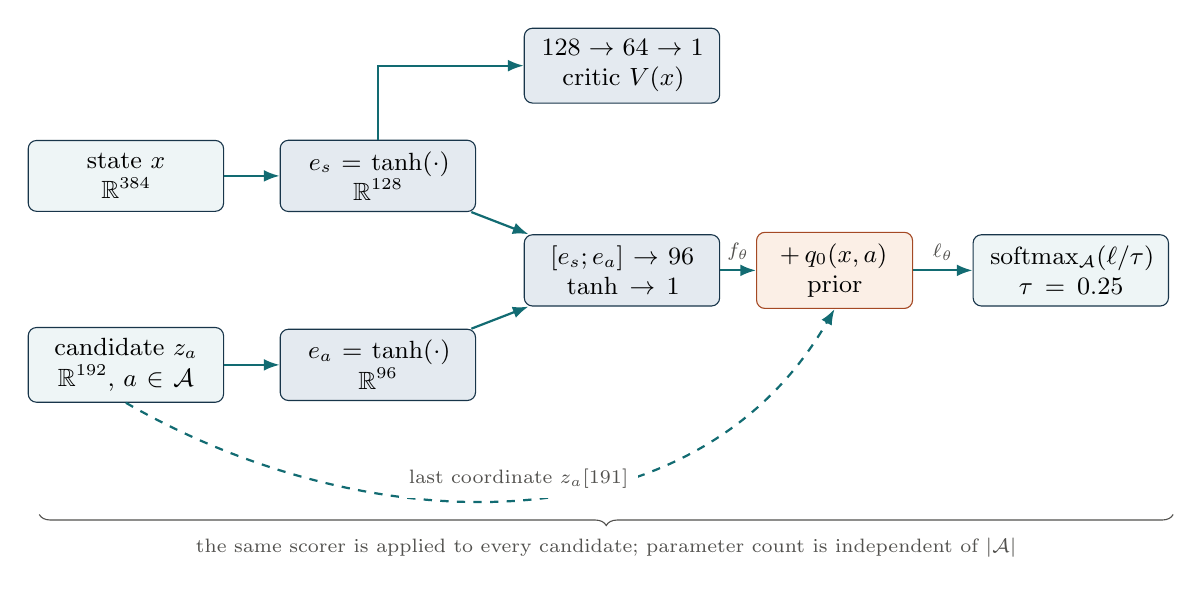
\begin{tikzpicture}[x=1cm,y=1cm]
  \node[box,text width=22mm] (x) at (0,1.2) {state $x$\\$\R^{384}$};
  \node[box,text width=22mm] (z) at (0,-1.2) {candidate $z_a$\\$\R^{192}$, $a\in\A$};
  \node[inkbox,text width=22mm] (es) at (3.2,1.2) {$e_s=\tanh(\cdot)$\\$\R^{128}$};
  \node[inkbox,text width=22mm] (ea) at (3.2,-1.2) {$e_a=\tanh(\cdot)$\\$\R^{96}$};
  \node[inkbox,text width=22mm] (h) at (6.3,0) {$[e_s;e_a]\to96$\\$\tanh\to1$};
  \node[warmbox,text width=17mm] (plus) at (9.0,0) {$+\,q_0(x,a)$\\prior};
  \node[box,text width=22mm] (pi) at (12.0,0) {$\softmax_{\A}(\ell/\tau)$\\$\tau=0.25$};
  \node[inkbox,text width=22mm] (v) at (6.3,2.6) {$128\to64\to1$\\critic $V(x)$};
  \draw[arr] (x) -- (es); \draw[arr] (z) -- (ea);
  \draw[arr] (es) -- (h); \draw[arr] (ea) -- (h);
  \draw[arr] (h) -- node[note,above]{$f_\theta$} (plus); \draw[arr] (plus) -- node[note,above]{$\ell_\theta$} (pi);
  \draw[arr] (es) |- (v);
  \draw[darr] (z.south) to[out=-30,in=-120] node[note,above,pos=.5,fill=white]{last coordinate $z_a[191]$} (plus.south);
  \draw[decorate,decoration={brace,amplitude=4pt,mirror},draw=muted] (-1.1,-3.1) -- (13.3,-3.1)
    node[midway,below=5pt,note]{the same scorer is applied to every candidate; parameter count is independent of $|\A|$};
\end{tikzpicture}
\caption{The deployed actor--critic. The final actor layer is initialized to
zero, so a fresh actor equals $\softmax(q_0/\tau)$. The optional
\code{matchup-v1} variant adds a bilinear term $u^\top(e_a\odot Me_s)$ to the
logit.}
\label{fig:network}
\end{figure}

\begin{table}[htbp]
\centering\small
\begin{tabular}{lrr}
\toprule
Module & Shape & Parameters \\
\midrule
State encoder & $384\to128$ & 49{,}280 \\
Action encoder & $192\to96$ & 18{,}528 \\
Actor head & $224\to96\to1$ & 21{,}697 \\
Critic head & $128\to64\to1$ & 8{,}321 \\
\midrule
\code{concat-v1} total (\textbf{deployed}) & & \textbf{97{,}826} \\
\code{matchup-v1} extra: $M$ ($128\to96$), $u$ ($96\to1$) & no bias & $12{,}288+96$ \\
\code{matchup-v1} total (rejected) & & 110{,}210 \\
Scout (Section~\ref{sec:scout}) & $384\to96\to938$ & 127{,}946 \\
\bottomrule
\end{tabular}
\caption{Parameter counts, checked by instantiating the classes. The scout's
output width equals the move vocabulary of the live format.}
\label{tab:params}
\end{table}

The \code{matchup-v1} migration loads every old tensor and zero-initializes
$u$, so migrated logits are exactly unchanged. That variant passed a
development panel (70 vs.\ 55 of 96) but tied its final panel 126--126 of
200, and was rejected. The deployed checkpoint (revision \code{893e35e3},
113 updates) is \code{concat-v1} with profile \code{strategic-v1}. It uses a
feedforward summary of history: no recurrence, no attention, and no search
inside the network.

\subsection{The tempered masked policy}
A checkpoint carries two temperatures in $[0.25,2]$: one for turns and one for
previews. The deployed value is $\tau=0.25$ for both. For a nonempty
candidate set the policy is
\begin{equation}
  \pi_\theta(a\mid x,\A)=
  \begin{cases}
    \dfrac{\exp(\ell_\theta(x,a)/\tau)}{\sum_{u\in\A}\exp(\ell_\theta(x,u)/\tau)}, &a\in\A,\\[1.5ex]
    0, &a\notin\A.
  \end{cases}
\label{eq:policy}
\end{equation}
The same $\tau$ is used for sampling, for stored log-probabilities, and for
the training loss. Inference scores only real candidates. Training pads
variable candidate sets and fills padded logits with the most negative finite
float. After division by $\tau<1$ that sentinel overflows to $-\infty$ in
float32. The categorical distribution handles this exactly, so padded
probabilities are exactly zero.

\begin{proposition}[Normalization, support and score function]
\label{prop:mask}
For finite logits, $\tau>0$ and a nonempty, parameter-independent set $\A$,
the policy~\eqref{eq:policy} sums to one, vanishes outside $\A$, and for
$a\in\A$ satisfies
\begin{equation}
  \nabla_\theta\log\pi_\theta(a\mid x,\A)
  =\frac1\tau\Big(\nabla_\theta\ell_\theta(x,a)
   -\sum_{u\in\A}\pi_\theta(u\mid x,\A)\nabla_\theta\ell_\theta(x,u)\Big).
\end{equation}
\end{proposition}
\begin{proof}
The denominator is a finite sum of positive terms, so the admissible
probabilities are positive and sum to one; the others are zero by definition.
The logarithm is $\ell_\theta(x,a)/\tau-\log\sum_u\exp(\ell_\theta(x,u)/\tau)$.
Differentiating the log-sum-exp gives the $\pi$-weighted average of
$\nabla\ell_\theta/\tau$.
\end{proof}

\intuition{A low temperature multiplies every logit gradient by $1/\tau=4$ and
sharpens the policy. Turn-temperature promotion was itself the project's
largest single measured improvement: the same weights at $\tau=0.25$ won 129
of 200 paired games against 95 at the previous setting.}

\begin{example}[Temperature changes the same preferences]
\label{ex:temperature}
For logits $(2.55,2.00,0.30)$, $\tau=1$ gives probabilities
$(0.594,0.343,0.063)$. The deployed $\tau=0.25$ gives
$(0.900,0.100,0.0001)$. Greedy play picks the first candidate in both cases.
These numbers are selection probabilities, not win probabilities.
\end{example}

\subsection{The learned residual as a tilt of the prior}
Fix an input and candidate set. Split the logit into the prior $q_0$ and the
learned residual $f_\theta=\ell_\theta-q_0$, and let
$q_\tau=\softmax(q_0/\tau)$. Then
\begin{equation}
  \pi_\theta(a)=\frac{q_\tau(a)\,e^{f_\theta(a)/\tau}}{Z},\qquad
  Z=\sum_uq_\tau(u)e^{f_\theta(u)/\tau}.
\end{equation}

\begin{proposition}[Variational form with temperature]
\label{prop:variational}
For a strictly positive $q_\tau$ and finite $f$ on a finite set, the
distribution $p^*\propto q_\tau e^{f/\tau}$ is the unique maximizer of
$\sum_ap(a)f(a)-\tau\KL(p\Vert q_\tau)$ over probability vectors $p$.
\end{proposition}
\begin{proof}
From $\log p^*=\log q_\tau+f/\tau-\log Z$,
\[
  \sum_ap(a)f(a)-\tau\KL(p\Vert q_\tau)=\tau\log Z-\tau\KL(p\Vert p^*).
\]
The right side is maximized, uniquely, where the KL divergence vanishes,
that is at $p=p^*$.
\end{proof}

\intuition{The policy behaves as if it maximized the learned residual
against a KL penalty toward the tempered prior, with penalty strength $\tau$.
At $\tau=0.25$ the prior is sharpened four-fold and the residual is also
amplified four-fold. The trainer never optimizes this objective explicitly,
and a large enough residual can overturn the prior completely.}

\paragraph{Permutation equivariance.} The scorer is applied independently to
each candidate. Permuting the candidate rows therefore permutes the logits
and probabilities in the same way. With a unique maximum, the greedy choice is
independent of list order. Exact ties fall back to the first index.

\source{\code{ActorCritic}, \code{Model.temperature}, \code{Model.predict}
and \code{enable_matchups} in \code{ml/model.py}; \code{Brain.decide} in
\code{ml/brain.py}.}

\section{The data recorded for every match}
\label{sec:data}

A learning system is only as trustworthy as its records. The recorder
answers four questions for every decision:
\begin{itemize}
  \item What did the player know?
  \item Which candidates were legal?
  \item With which probabilities, under which exact checkpoint, was one
    sampled?
  \item What happened afterwards?
\end{itemize}
The current format is \emph{recorder~3}.

\subsection{Anatomy of an episode}
Figure~\ref{fig:episode} shows one episode as stored in the \code{episodes}
table. An episode is a JSON document of four parts: a header, the conditions
of collection, the decision steps, and a terminal section.

\begin{figure}[htbp]
\centering
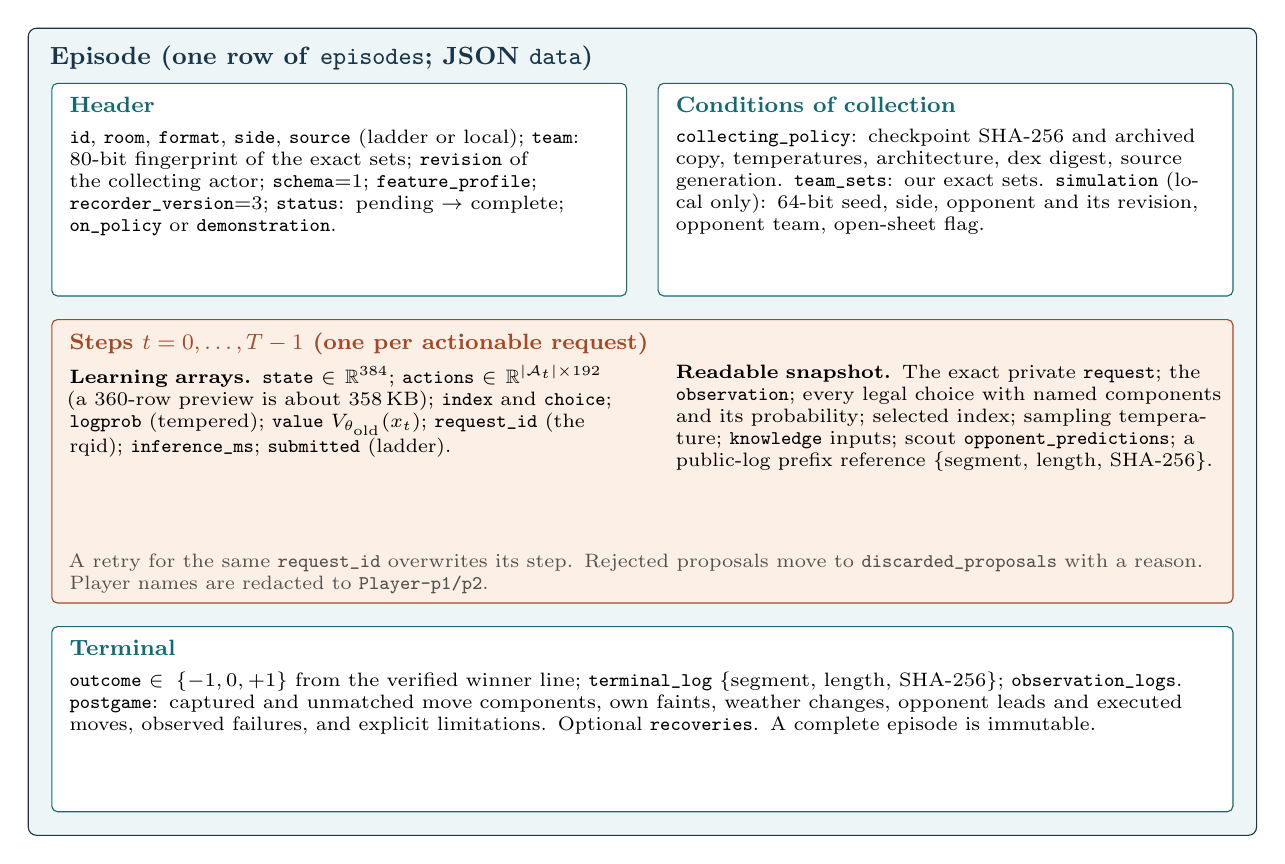
\begin{tikzpicture}[x=1cm,y=1cm,
  field/.style={font=\scriptsize,align=left,anchor=north west,text width=#1},
  field/.default=6.6cm]
  % outer episode
  \draw[draw=ink,rounded corners=3pt,fill=pale] (0,0) rectangle (15.6,-10.25);
  \node[font=\small\bfseries,text=ink,anchor=north west] at (0.15,-0.1) {Episode (one row of \code{episodes}; JSON \code{data})};
  % header
  \draw[draw=accent,fill=white,rounded corners=2pt] (0.3,-0.7) rectangle (7.6,-3.4);
  \node[font=\footnotesize\bfseries,anchor=north west,text=accent] at (0.4,-0.75) {Header};
  \node[field] at (0.4,-1.15) {\code{id}, \code{room}, \code{format}, \code{side}, \code{source}
    (ladder or local); \code{team}: 80-bit fingerprint of the exact sets;
    \code{revision} of the collecting actor; \code{schema}=1;
    \code{feature_profile}; \code{recorder_version}=3; \code{status}:
    pending $\to$ complete; \code{on_policy} or \code{demonstration}.};
  % collecting policy
  \draw[draw=accent,fill=white,rounded corners=2pt] (8.0,-0.7) rectangle (15.3,-3.4);
  \node[font=\footnotesize\bfseries,anchor=north west,text=accent] at (8.1,-0.75) {Conditions of collection};
  \node[field] at (8.1,-1.15) {\code{collecting_policy}: checkpoint SHA-256 and archived
    copy, temperatures, architecture, dex digest, source generation.
    \code{team_sets}: our exact sets. \code{simulation} (local only): 64-bit seed,
    side, opponent and its revision, opponent team, open-sheet flag.};
  % steps
  \draw[draw=seriesB!70!black,fill=warm,rounded corners=2pt] (0.3,-3.7) rectangle (15.3,-7.3);
  \node[font=\footnotesize\bfseries,anchor=north west,text=seriesB!70!black] at (0.4,-3.75) {Steps $t=0,\dots,T-1$ (one per actionable request)};
  \node[field=7.0cm] at (0.4,-4.15) {\textbf{Learning arrays.} \code{state} $\in\R^{384}$;
    \code{actions} $\in\R^{|\A_t|\times192}$ (a 360-row preview is about 358\,KB);
    \code{index} and \code{choice}; \code{logprob} (tempered);
    \code{value} $V_{\theta_{\mathrm{old}}}(x_t)$; \code{request_id} (the rqid);
    \code{inference_ms}; \code{submitted} (ladder).};
  \node[field=7.0cm] at (8.1,-4.15) {\textbf{Readable snapshot.} The exact private \code{request};
    the \code{observation}; every legal choice with named components and its
    probability; selected index; sampling temperature; \code{knowledge}
    inputs; scout \code{opponent_predictions}; a public-log prefix reference
    \{segment, length, SHA-256\}.};
  \node[font=\scriptsize,text=muted,anchor=north west,text width=14.6cm] at (0.4,-6.55)
    {A retry for the same \code{request_id} overwrites its step. Rejected proposals move to
     \code{discarded_proposals} with a reason. Player names are redacted to \code{Player-p1/p2}.};
  % terminal
  \draw[draw=accent,fill=white,rounded corners=2pt] (0.3,-7.6) rectangle (15.3,-9.95);
  \node[font=\footnotesize\bfseries,anchor=north west,text=accent] at (0.4,-7.65) {Terminal};
  \node[field=14.6cm] at (0.4,-8.05) {\code{outcome} $\in\{-1,0,+1\}$ from the
    verified winner line; \code{terminal_log} \{segment, length, SHA-256\};
    \code{observation_logs}. \code{postgame}: captured and unmatched move components,
    own faints, weather changes, opponent leads and executed moves, observed
    failures, and explicit limitations. Optional \code{recoveries}. A complete
    episode is immutable.};
\end{tikzpicture}
\caption{The recorder-3 episode. Learning uses the orange arrays; auditing and
replay use the snapshot. For the last 20 ladder games the median document was
1.30\,MB (range 0.73--2.06\,MB). In a 7-step game, feature arrays took 750\,KB
and snapshots 440\,KB of 1.20\,MB.}
\label{fig:episode}
\end{figure}

\subsection{Tables}
The store is one SQLite database in write-ahead-log mode. Its tables are listed
in Table~\ref{tab:sqlite}. Jobs carry a persistent identity, status, attempt
count and a lease, which is how the three lanes of
Section~\ref{sec:pipeline} share work safely.

\begin{table}[htbp]
\centering\small
\begin{tabularx}{\linewidth}{>{\raggedright\arraybackslash}p{0.2\linewidth} X r}
\toprule
Table & Contents & Rows (M-C) \\
\midrule
\code{episodes} & Header columns plus the JSON document above & 14{,}137 complete \\
\code{jobs} & Collector, learner, feed and evaluator jobs with leases & --- \\
\code{public_battles} & Sanitized public logs, unique by digest & 12{,}573 \\
\code{scout_samples} & Pre-turn public vectors with executed-move labels & 192{,}835 \\
\code{research_teams}, \code{documents} & Attributed tournament sets and prose & --- \\
\code{team_metadata}, \code{feed_state} & Team versions; daily feed bookkeeping & --- \\
\bottomrule
\end{tabularx}
\caption{SQLite schema. Counts are a read-only snapshot taken on 9 October
2026 at about 20:15\,UTC, while collection was still running (database
18.4\,GB). Of the complete M-C episodes, 854 are recorded ladder games
(353--501) and 13{,}283 are local self-play games (9{,}010--4{,}273); there
are no ties. The recorded ladder count also includes browser games played in
model mode after the 847-game campaign stopped.}
\label{tab:sqlite}
\end{table}

\subsection{What makes a record usable for learning}
Before any gradient step, each candidate episode passes
\code{trajectory_issues}. An episode is excluded, not repaired, if any check
fails:
\begin{enumerate}
  \item It is not complete, has another format, revision, schema or feature
    profile, or its outcome is outside $\{-1,0,1\}$.
  \item Any ladder step was proposed but never submitted.
  \item Any array has the wrong shape or a non-finite value, or any stored
    log-probability exceeds $10^{-6}$.
  \item The snapshot's probabilities do not sum to one, or
    $p[\text{index}]\ne e^{\text{logprob}}$ (relative tolerance $10^{-5}$).
  \item The snapshot's choices differ from \code{legal_choices} of its own
    stored request.
  \item A log-prefix digest fails, a step contains future or terminal lines,
    a request is credited twice, or the terminal log lacks a win or tie line.
\end{enumerate}
A second check recomputes every stored log-probability under the archived
collecting checkpoint (Section~\ref{sec:likelihood}). Excluded episodes are
never marked consumed, so a persistent defect stays visible in later batch
reports rather than disappearing silently.

\subsection{Games played by search}
A browser game decided by search writes no \code{episodes} row. Its actions
were not sampled from $\pi_\theta$, so storing them as PPO samples would give
false importance ratios (Section~\ref{sec:ratios}). The runner logs each
decision, with its request, choice and search statistics, to a private
per-run ledger. At the end of the game, the sanitized public log enters
\code{public_battles} as an \code{own-live-game} and yields scout labels.

\subsection{Storage lifecycle and budget}
Data has a bounded lifetime, shown in Figure~\ref{fig:storage}. Each candidate
freezes the inference inputs it was evaluated with: research teams, documents,
species and move support, and scout weights. These are stored as a
content-addressed, read-only snapshot. Completed snapshots are gzip-archived
every 900\,s, with byte-count and SHA-256 verification, so they stay
reproducible. A storage budget limits optional work.

\begin{figure}[htbp]
\centering
\resizebox{\linewidth}{!}{%
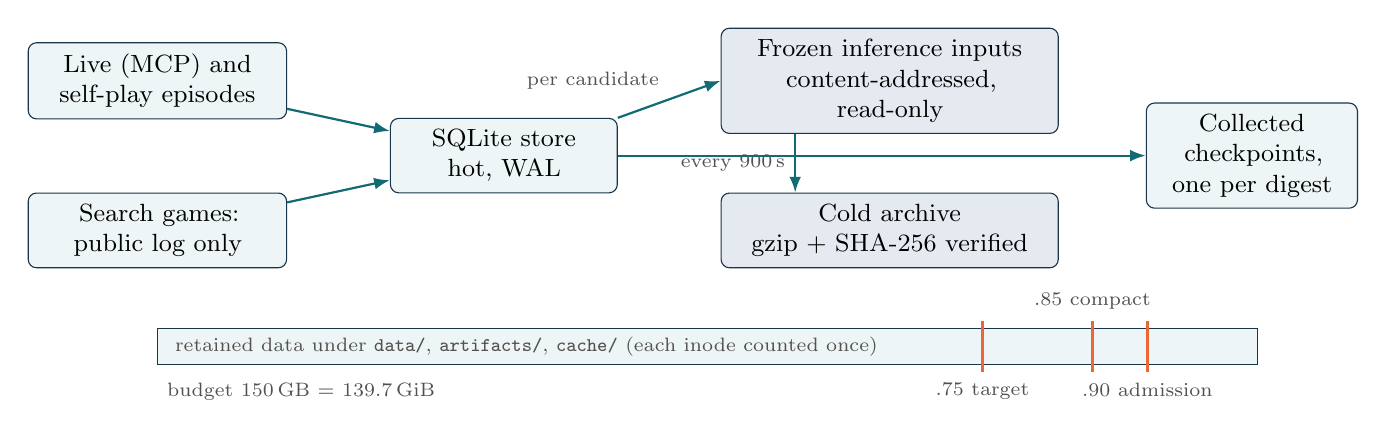
\begin{tikzpicture}[x=1cm,y=1cm]
  \node[box,text width=30mm] (src) at (0,0) {Live (MCP) and\\self-play episodes};
  \node[box,text width=30mm] (pub) at (0,-1.9) {Search games:\\public log only};
  \node[box,text width=26mm] (db) at (4.4,-0.95) {SQLite store\\hot, WAL};
  \node[inkbox,text width=40mm] (snap) at (9.3,0) {Frozen inference inputs\\content-addressed, read-only};
  \node[inkbox,text width=40mm] (cold) at (9.3,-1.9) {Cold archive\\gzip + SHA-256 verified};
  \node[box,text width=24mm] (ck) at (13.9,-0.95) {Collected\\checkpoints,\\one per digest};
  \draw[arr] (src) -- (db); \draw[arr] (pub) -- (db);
  \draw[arr] (db.north east) -- node[note,above left]{per candidate} (snap.west);
  \draw[arr] ([xshift=-12mm]snap.south) -- node[note,left]{every 900\,s} ([xshift=-12mm]cold.north);
  \draw[arr] (db.east) -- (ck.west);
  % budget bar
  \begin{scope}[yshift=-3.6cm]
    \fill[pale] (0,0) rectangle (13.97,0.45);
    \draw[draw=ink] (0,0) rectangle (13.97,0.45);
    \foreach \f/\l in {0.75/{.75: compaction target},0.85/{.85: compaction trigger},0.90/{.90: optional work stops}}{
      \draw[very thick,draw=seriesB] (13.97*\f,-0.1) -- (13.97*\f,0.55);
    }
    \node[note,anchor=north] at (13.97*0.75,-0.12) {.75 target};
    \node[note,anchor=south] at (13.97*0.85,0.57) {.85 compact};
    \node[note,anchor=north] at (13.97*0.90,-0.12) {.90 admission};
    \node[note,anchor=west] at (0.1,0.225) {retained data under \code{data/}, \code{artifacts/}, \code{cache/} (each inode counted once)};
    \node[note,anchor=north west] at (0,-0.12) {budget 150\,GB = 139.7\,GiB};
  \end{scope}
\end{tikzpicture}}
\caption{Data lifecycle and the storage budget. Above 90\% of the budget,
collection, learning and evaluation defer. Above 85\%, finished candidates'
input snapshots are compacted down to 75\%. Collecting checkpoints are kept
once per digest, so every recorded likelihood can be recomputed.}
\label{fig:storage}
\end{figure}

\source{\code{ml/storage.py} (schema, fingerprint, collected checkpoints);
\code{ml/brain.py} and \code{ml/recording.py} (steps and snapshots);
\code{ml/postgame.py}; \code{ml/data_quality.py}; \code{ml/input_snapshot.py};
\code{ml/data_budget.py}; \code{docs/cold-input-archiving.md};
\code{docs/model-storage.md}.}

\section{Learning from outcomes: policy gradients, GAE and PPO}
\label{sec:learning}

\subsection{Reward and objective}
For a completed episode with $T$ recorded decisions, let $Y\in\{-1,0,1\}$ be
loss, tie or win from our side. The reward is terminal only:
$r_t=0$ for $t<T-1$ and $r_{T-1}=Y$. With $\gamma=0.99$,
\begin{equation}
  G_t=\sum_{j=t}^{T-1}\gamma^{j-t}r_j=\gamma^{\,T-1-t}\,Y.
\end{equation}
With $\gamma=1$, $\E[Y]=\Prob(\mathrm{win})-\Prob(\mathrm{loss})
=2\Prob(\mathrm{win})+\Prob(\mathrm{tie})-1$. When ties are absent, as in every
recorded M-C game, maximizing $\E[Y]$ is the same as maximizing win
probability. With $\gamma<1$, the same outcome is worth less after a longer
game, so training mildly prefers shorter wins and longer losses. The promotion
gate counts raw wins. The two criteria are related but not identical.

For a fixed policy, the history-conditioned value, action value and advantage
are $V^\pi(h_t)=\E_\pi[G_t\mid h_t]$,
$Q^\pi(h_t,a)=\E_\pi[G_t\mid h_t,a_t=a]$ and $A^\pi=Q^\pi-V^\pi$. The critic
approximates $V^\pi$ through compressed features. Its output is unbounded and
is not a calibrated win probability.

\subsection{The policy-gradient identity on histories}
\begin{theorem}[Finite-horizon likelihood-ratio gradient]
\label{thm:gradient}
Assume a finite trajectory space and a finite horizon $T$, padding terminated
trajectories with zero-reward absorbing steps. Assume bounded rewards, a
differentiable policy with parameter-independent support on each history, and
environment and opponent kernels that do not depend on $\theta$. Let
$J(\theta)=\E_\theta[\sum_{t<T}\gamma^tr_t]$. Then
\begin{equation}
  \nabla_\theta J(\theta)=
  \E_\theta\Big[\sum_{t=0}^{T-1}\gamma^tG_t\,
       \nabla_\theta\log\pi_\theta(a_t\mid h_t)\Big],
\label{eq:gradient}
\end{equation}
and $G_t$ may be replaced by $G_t-B(h_t)$ for any action-independent baseline
$B$ without changing the expectation.
\end{theorem}
\begin{proof}
A trajectory's probability factors into initial, transition and policy terms.
Only the policy terms depend on $\theta$, so
$\nabla\log p_\theta(\tau)=\sum_t\nabla\log\pi_\theta(a_t\mid h_t)$.
Differentiating the finite expectation gives $\E[R(\tau)\nabla\log
p_\theta(\tau)]$. A reward earned before $a_t$ is determined by $h_t$, and
$\E[\nabla\log\pi_\theta(a_t\mid h_t)\mid h_t]=\sum_a\nabla\pi_\theta(a\mid
h_t)=\nabla1=0$. Those cross terms therefore vanish, which leaves
$\sum_{j\ge t}\gamma^jr_j=\gamma^tG_t$. The same zero-mean identity removes the
baseline.
\end{proof}

\intuition{An action gains probability when the outcome that follows it is
better than expected for that situation. The theorem needs no Markov
assumption on the hashed features, because it is stated on histories. It does
need the recorded action to have actually been sampled from $\pi_\theta$.
This is why search decisions are never PPO data.}

\caveat{The implemented surrogate averages decision samples equally and omits
the $\gamma^t$ factor. It is therefore a standard heuristic related to
Equation~\eqref{eq:gradient}, not an unbiased estimator of $\nabla J$
\citep{policygradient,ppo,gae}. Opponent kernels are not fixed in self-play
either: the \code{self} opponent is a frozen snapshot of the incumbent, which
is fixed within a batch but changes after each promotion.}

\subsection{Generalized advantage estimation}
Using the collecting critic's stored values $V_t$, and $V_T=0$,
\begin{align}
  \delta_t&=r_t+\gamma V_{t+1}-V_t,\qquad
  \widehat A_t=\delta_t+\gamma\lambda\widehat A_{t+1},\qquad \widehat A_T=0,\qquad\lambda=0.95,\\
  \widehat R_t&=\widehat A_t+V_t.
\label{eq:gae}
\end{align}
Figure~\ref{fig:gae} shows how the recursion runs backward through one
episode.

\begin{figure}[htbp]
\centering
\resizebox{\linewidth}{!}{%
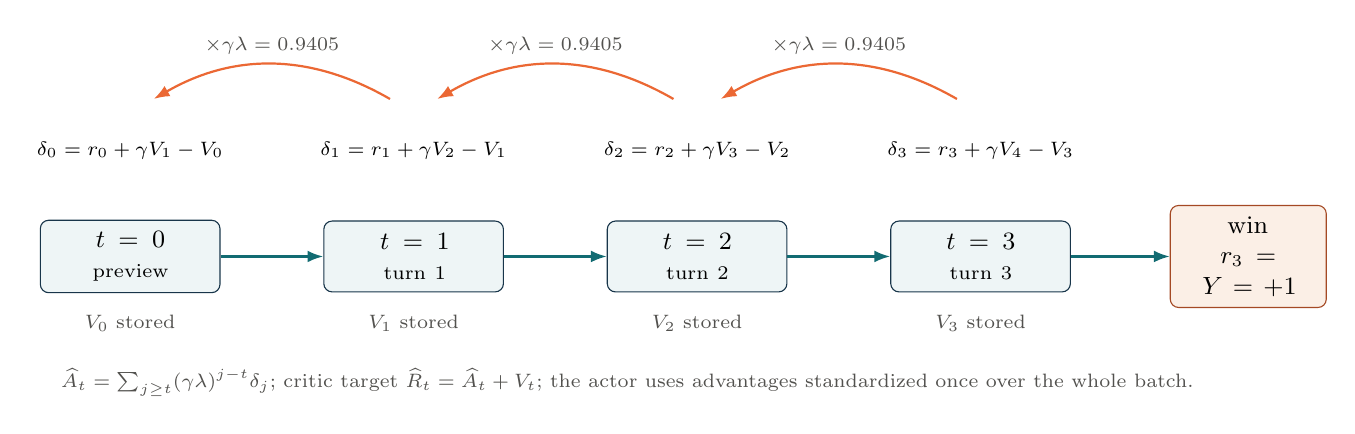
\begin{tikzpicture}[x=1cm,y=1cm]
  \foreach \i/\lab in {0/{preview},1/{turn 1},2/{turn 2},3/{turn 3}}{
    \node[box,text width=20mm] (s\i) at (3.6*\i,0) {$t=\i$\\\scriptsize\lab};
    \node[note] at (3.6*\i,-0.85) {$V_\i$ stored};
  }
  \node[warmbox,text width=17mm] (end) at (14.2,0) {win\\$r_3=Y=+1$};
  \foreach \i/\j in {0/1,1/2,2/3}{ \draw[arr] (s\i) -- (s\j); }
  \draw[arr] (s3) -- (end);
  \foreach \i in {0,1,2,3}{
    \node[font=\scriptsize] (d\i) at (3.6*\i,1.35) {$\delta_\i=r_\i+\gamma V_{\the\numexpr\i+1\relax}-V_\i$};
  }
  \foreach \i/\j in {3/2,2/1,1/0}{
    \draw[-{Latex[length=2mm]},thick,draw=seriesB] (3.6*\i-0.3,2.0) to[out=150,in=30]
      node[note,above]{$\times\gamma\lambda=0.9405$} (3.6*\j+0.3,2.0);
  }
  \node[font=\scriptsize,text=muted,align=left,anchor=west] at (-1.0,-1.6)
   {$\widehat A_t=\sum_{j\ge t}(\gamma\lambda)^{j-t}\delta_j$; critic target $\widehat R_t=\widehat A_t+V_t$;
    the actor uses advantages standardized once over the whole batch.};
\end{tikzpicture}}
\caption{GAE on a four-decision episode with a terminal win. Only the last
residual contains the reward. Each earlier advantage adds its own residual to
the next advantage, discounted by $\gamma\lambda$.}
\label{fig:gae}
\end{figure}

\begin{proposition}[GAE expansion and the Monte Carlo endpoint]
\label{prop:gae}
The recurrence~\eqref{eq:gae} gives
$\widehat A_t=\sum_{j=t}^{T-1}(\gamma\lambda)^{j-t}\delta_j$. If $\lambda=1$
and $V_T=0$, then $\widehat A_t=G_t-V_t$.
\end{proposition}
\begin{proof}
Unroll the recurrence backward from $\widehat A_T=0$, or argue by induction
from $t=T-1$. With $\lambda=1$, the $+\gamma V_{j+1}$ in each residual cancels
the $-V_{j+1}$ in the next one after discounting. What remains is the
discounted rewards, $-V_t$, and $\gamma^{T-t}V_T=0$.
\end{proof}

\begin{example}[Two decisions ending in a win]
With $(V_0,V_1)=(0.20,0.30)$ and $(r_0,r_1)=(0,1)$: $\delta_1=0.70$,
$\delta_0=0.99(0.30)-0.20=0.097$, $\widehat A_1=0.70$, and
$\widehat A_0=0.097+0.9405(0.70)=0.75535$. The critic targets are
$(0.95535,1.00)$; the Monte Carlo target for $t=0$ would be 0.99.
\end{example}

\subsection{Stored probabilities and importance ratios}
\label{sec:ratios}
For a step collected by revision $\theta_{\mathrm{old}}$, PPO uses
\begin{equation}
  \rho_t(\theta)=\frac{\pi_\theta(a_t\mid x_t,\A_t)}{\pi_{\theta_{\mathrm{old}}}(a_t\mid x_t,\A_t)}
  =\exp\big(\log\pi_\theta(a_t\mid x_t,\A_t)-\mathrm{storedLogProb}_t\big),
\end{equation}
with both policies tempered as in Equation~\eqref{eq:policy}.

\begin{proposition}[Conditional importance identity]
\label{prop:importance}
At a fixed stored input and candidate set, if the old policy $p$ is positive
wherever the new policy $q$ is, then $\E_{a\sim p}[(q(a)/p(a))f(a)]=\E_{a\sim
q}[f(a)]$ for every real $f$.
\end{proposition}
\begin{proof}
Write the left side as $\sum_ap(a)\,q(a)f(a)/p(a)$ and cancel $p(a)$ on its
support. The support assumption means no term with positive $q$-mass is lost.
\end{proof}

This corrects the action choice at fixed inputs only, not the whole
trajectory distribution. It is wrong when the action was really chosen by
greedy play, a human, search, or an unknown policy. Rejections add a further
subtlety. The stored likelihood is the probability of the \emph{proposal}. If
hidden restrictions reject some proposals and only accepted ones survive, the
executed action follows the proposal policy conditioned on acceptance. The
recorder therefore keeps rejected proposals separately, and accepts a step
only after its submission is confirmed.

\subsection{Collecting-likelihood validation}
\label{sec:likelihood}
Before training, the learner reloads the parent (collecting) weights and
recomputes every stored step's tempered log-probability. Any episode with a
step where the recomputed and stored values differ by more than
$\eta=10^{-4}$ is excluded.

\begin{proposition}[What the likelihood check guarantees]
\label{prop:likelihood}
Suppose every retained step satisfies
$|\log\pi_{\theta_{\mathrm{old}}}(a_t)-\mathrm{storedLogProb}_t|\le\eta$, with
the left side recomputed from the stored inputs. Then for every $\theta$ the
ratio used in training equals the exact ratio times $e^{\epsilon_t}$ with
$|\epsilon_t|\le\eta$. For $\eta=10^{-4}$, the relative ratio error is at most
$e^{\eta}-1\approx1.00005\times10^{-4}$.
\end{proposition}
\begin{proof}
Write $\epsilon_t=\log\pi_{\theta_{\mathrm{old}}}(a_t)-\mathrm{storedLogProb}_t$.
Then $\exp(\log\pi_\theta-\mathrm{storedLogProb})
=\exp(\log\pi_\theta-\log\pi_{\theta_{\mathrm{old}}})e^{\epsilon_t}$, and
$|\epsilon_t|\le\eta$ by assumption.
\end{proof}

\intuition{The check certifies more than arithmetic. A trajectory whose
features, candidate list, checkpoint or temperature changed after recording
would fail it. The six most recent learner jobs had a maximum discrepancy of
$1.9\times10^{-6}$. The check cannot certify that the recorded inputs were
themselves a faithful observation; Section~\ref{sec:game} covers that
separately.}

\subsection{The optimized PPO loss}
Advantages are standardized once over the whole batch, before any epoch:
$\widetilde A_t=(\widehat A_t-\overline A)/(s_A+10^{-8})$ when the batch has
more than one sample and $s_A>10^{-6}$. Here $s_A$ is the population
standard deviation. Each minibatch $\mathcal B$ of size $B$ also carries phase
weights $\omega_t=w_t/\overline w_{\mathcal B}$, where $w_t$ is the preview
training weight ($1\le w\le16$) for preview steps and 1 otherwise. The
minimized loss is
\begin{equation}
  \mathcal L(\theta)=\frac1B\sum_{t\in\mathcal B}\omega_t\Big[
   -\min\!\big(\rho_t\widetilde A_t,\clip(\rho_t,0.8,1.2)\widetilde A_t\big)
   +0.5\big(V_\theta(x_t)-\widehat R_t\big)^2
   -c_H\,H\big(\pi_\theta(\cdot\mid x_t,\A_t)\big)\Big].
\label{eq:loss}
\end{equation}
The entropy is that of the tempered distribution, and the value loss is not
clipped. The deployed configuration is: entropy coefficient $c_H=0.01$; preview
weight 1 (so $\omega_t\equiv1$); Adam with learning rate $3\cdot10^{-4}$;
minibatches of 32 drawn by a seeded permutation; four epochs; global
gradient-norm clip 0.5; target KL 0.03. A non-finite loss aborts before any
checkpoint is written. Each training call produces a new revision UUID and
increments the update counter once.

\begin{proposition}[What clipping bounds]
\label{prop:clip}
For a fixed advantage $A$ and positive ratio $\rho$,
\[
  \min(\rho A,\clip(\rho,1-\epsilon,1+\epsilon)A)=
  \begin{cases}A\min(\rho,1+\epsilon),&A\ge0,\\A\max(\rho,1-\epsilon),&A<0,\end{cases}
\]
and this is never larger than the unclipped term $\rho A$.
\end{proposition}
\begin{proof}
For $A\ge0$ multiplication by $A$ preserves order, so the minimum picks the
smaller of $\rho$ and $\clip(\rho)$. That is $\min(\rho,1+\epsilon)$, because
clipping from below never lowers $\rho$. For $A<0$ the order reverses. The
minimum picks the larger of the two, which is $\max(\rho,1-\epsilon)$. Taking
a minimum with $\rho A$ cannot exceed $\rho A$.
\end{proof}

\begin{example}[A clipped update]
If $\pi_{\mathrm{old}}(a)=0.20$, $\pi_\theta(a)=0.30$ and $A=0.70$, then
$\rho=1.5$. The unclipped term is 1.05; the clipped term is
$1.2(0.70)=0.84$. With $A=-0.70$ and $\rho=0.5$ the clipped term is
$0.8(-0.70)=-0.56$, not $-0.35$.
\end{example}

The proposition does not keep every ratio within $[0.8,1.2]$, does not enforce
a KL constraint, and does not lower-bound win-rate improvement
\citep{ppo,trpo}. The KL stop below is the implementation's coarse trust
region.

\subsection{The KL early stop}
After each full epoch, the learner evaluates the whole batch at the current
parameters and computes
\begin{equation}
  \widehat{\KL}=\frac1N\sum_{i=1}^N\big[(\rho_i-1)-\log\rho_i\big],
  \label{eq:k3}
\end{equation}
where $\rho_i$ is the ratio at the stored action. If $\widehat{\KL}>0.03$, the
remaining epochs are skipped. The updates from the epoch that crossed the
threshold are \emph{kept}.

\begin{proposition}[The KL estimator]
\label{prop:k3}
Fix a state, an old policy $p$ and a new policy $q$ with the same support, and
let $\rho(a)=q(a)/p(a)$. Then each term $(\rho-1)-\log\rho$ is non-negative,
and $\E_{a\sim p}[(\rho(a)-1)-\log\rho(a)]=\KL(p\Vert q)$. Consequently, if
the stored actions were sampled from the old policy, Equation~\eqref{eq:k3} is
an unbiased estimate of the average $\KL(\pi_{\mathrm{old}}\Vert\pi_\theta)$
over the batch's stored states.
\end{proposition}
\begin{proof}
For $u>0$, $u-1-\log u\ge0$, with equality only at $u=1$, because $\log u\le
u-1$. Next, $\E_p[\rho]=\sum_aq(a)=1$, so $\E_p[\rho-1]=0$, and
$\E_p[-\log\rho]=\sum_ap(a)\log(p(a)/q(a))=\KL(p\Vert q)$. Averaging over
states with their stored actions preserves unbiasedness, by linearity.
\end{proof}

\caveat{The estimator is unbiased for $\KL(\text{old}\Vert\text{new})$
(\citealp{klapprox}). The check runs only between epochs, so the returned
candidate can exceed 0.03 by up to one epoch's movement. Recent production
batches stopped at final-epoch values between 0.012 and 0.017, so none
triggered the stop. The statistic is still computed on the same samples used
for the gradient, so it is a training-set diagnostic rather than a held-out
one.}

\subsection{Demonstrations}
For explicitly labelled demonstrations $(x_t,\A_t,a_t^*)$, a separate training
call minimizes
\begin{equation}
  \mathcal L_{\mathrm{BC}}(\theta)=-\frac1B\sum_t\omega_t\log\pi_\theta(a_t^*\mid x_t,\A_t),
\end{equation}
the weighted conditional log-likelihood. There is no ratio, entropy or value
term, and no collecting-likelihood check. The shared state encoder still
changes, so the critic moves too. Imitating a weak teacher does not make the
learner an expert.

\source{\code{Model.train} (eligibility, GAE, likelihood validation,
standardization, loss, KL stop, saving) in \code{ml/model.py};
\code{RolloutBatcher} in \code{ml/batching.py}; \code{trajectory_issues} in
\code{ml/data_quality.py}; \code{LearningConfig} in \code{ml/continuous.py}.}

\section{The training pipeline on CPU and Apple MPS}
\label{sec:pipeline}

\subsection{From a game to a deployed checkpoint}
Figure~\ref{fig:pipeline} traces one unit of experience through the pipeline.
Each arrow is a durable hand-off: a SQLite row, a job, a file written by
atomic replacement, or a lease. A crash at any point therefore leaves either
the old state or the new one, and the next supervisor tick resumes from it.

\begin{figure}[htbp]
\centering
\resizebox{\linewidth}{!}{%
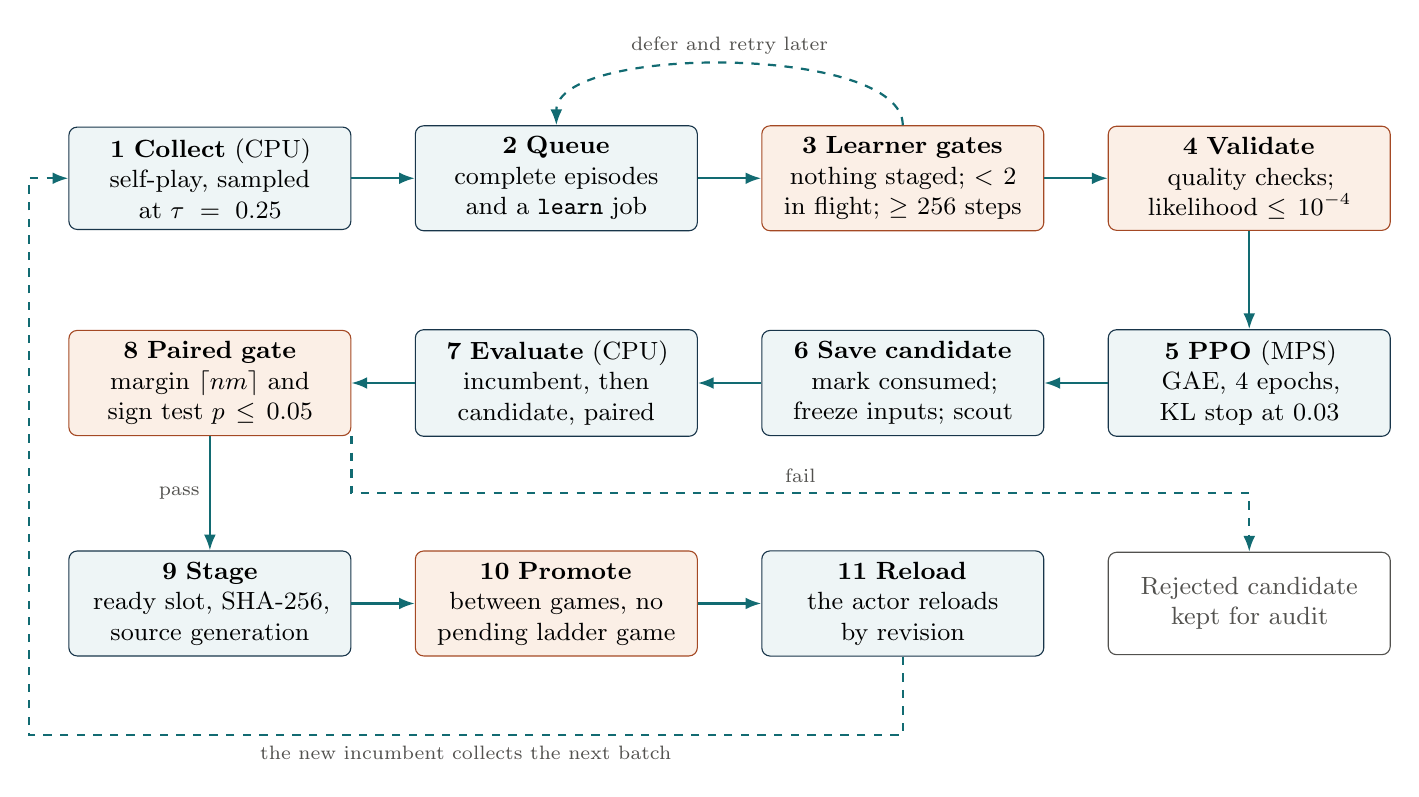
\begin{tikzpicture}[x=1cm,y=1cm,
  pstep/.style={box,text width=33mm,minimum height=13mm},
  pgate/.style={warmbox,text width=33mm,minimum height=13mm}]
  \node[pstep] (c) at (0,0) {\textbf{1 Collect} (CPU)\\self-play, sampled\\at $\tau=0.25$};
  \node[pstep] (q) at (4.4,0) {\textbf{2 Queue}\\complete episodes\\and a \code{learn} job};
  \node[pgate] (g) at (8.8,0) {\textbf{3 Learner gates}\\nothing staged; $<2$\\in flight; $\ge256$ steps};
  \node[pgate] (v) at (13.2,0) {\textbf{4 Validate}\\quality checks;\\likelihood $\le10^{-4}$};
  \node[pstep] (p) at (13.2,-2.6) {\textbf{5 PPO} (MPS)\\GAE, 4 epochs,\\KL stop at 0.03};
  \node[pstep] (s) at (8.8,-2.6) {\textbf{6 Save candidate}\\mark consumed;\\freeze inputs; scout};
  \node[pstep] (e) at (4.4,-2.6) {\textbf{7 Evaluate} (CPU)\\incumbent, then\\candidate, paired};
  \node[pgate] (pg) at (0,-2.6) {\textbf{8 Paired gate}\\margin $\lceil nm\rceil$ and\\sign test $p\le0.05$};
  \node[pstep] (r) at (0,-5.4) {\textbf{9 Stage}\\ready slot, SHA-256,\\source generation};
  \node[pgate] (pr) at (4.4,-5.4) {\textbf{10 Promote}\\between games, no\\pending ladder game};
  \node[pstep] (d) at (8.8,-5.4) {\textbf{11 Reload}\\the actor reloads\\by revision};
  \node[box,text width=33mm,minimum height=13mm,draw=muted,fill=white] (rej) at (13.2,-5.4) {\textcolor{muted}{Rejected candidate}\\\textcolor{muted}{kept for audit}};
  \draw[arr] (c)--(q); \draw[arr] (q)--(g); \draw[arr] (g)--(v); \draw[arr] (v)--(p);
  \draw[arr] (p)--(s); \draw[arr] (s)--(e); \draw[arr] (e)--(pg);
  \draw[arr] (pg)-- node[note,left]{pass} (r); \draw[arr] (r)--(pr); \draw[arr] (pr)--(d);
  \draw[darr] (pg.south east) |- node[note,above,pos=.75]{fail} (13.2,-4.0) -- (rej.north);
  \draw[darr] (d.south) -- ++(0,-1.0) -| node[note,below,pos=.25]{the new incumbent collects the next batch} (-2.3,0) -- (c.west);
  \draw[darr] (g.north) to[out=90,in=90,looseness=.6] node[note,above]{defer and retry later} (q.north);
\end{tikzpicture}}
\caption{The lifecycle of experience. Orange boxes are gates that can stop
the flow. Steps 1 and 7 run on the CPU, step 5 on the MPS GPU. Promotion
(step 10) is called by the player between games, never by a worker. Episodes
are marked consumed when the candidate is saved, before it is evaluated, so
``trained'' means \emph{used for a candidate}, not \emph{deployed}.}
\label{fig:pipeline}
\end{figure}

\paragraph{Collection.} The collector snapshots the incumbent and freezes
its inference inputs. It then plays \code{simulation_games} games (default
24) in waves of spawned one-thread processes. Each process drives the
official \code{BattleStream} through \code{simulator.cjs} and observes only
its own player stream. The \code{ladder-v1} curriculum cycles the opponent
through
\[
  (\text{self},\ \text{tactical},\ \text{heuristic},\ \text{self},\ \text{tactical},\ \text{random},\ \text{heuristic},\ \text{tactical}),
\]
with index $(\lfloor i/|\text{teams}|\rfloor+\text{seed})\bmod8$, so one
opponent completes a sweep of the team pool before the next takes over. In
each cycle that is 2/8 self-play against the frozen incumbent, 3/8 tactical,
2/8 heuristic and 1/8 random. Open team sheets are drawn with probability
0.08. Sides alternate as $(i+\lfloor i/|\text{teams}|\rfloor)\bmod2$. Seeds
are 64-bit, split into four 16-bit words. An earlier encoding used only 16
bits and was retired.

\paragraph{Learning.} The learner applies the gates of step~3, the
validation of step~4 and the loss of Section~\ref{sec:learning}. It runs on
the device chosen by \code{backend_for}. In automatic mode MPS is chosen only
if its benchmarked time is at most 0.85 of the CPU time. Any device error
retrains the same batch from the incumbent on the CPU. For the strategic
profiles the learner then refreshes the candidate's embedded
\code{strategy_knowledge} with new ladder postgame counts. It also trains the
public-move scout on the same lane.

\paragraph{Evaluation.} Incumbent and candidate are frozen CPU snapshots.
They play $n$ games each (60 in the deployed configuration; default 20), on
seeds $s_0+100000+i$ derived from the job identity. Actions are sampled at the
checkpoint temperature. Both panels face the same frozen \code{self} snapshot
and the same frozen inputs. Panels resume after interruption. The evaluator
abandons a plan if the source generation, parent revision or candidate hash
has changed.

\subsection{Three lanes on one laptop}
Figure~\ref{fig:lanes} shows how the work is shared out in time. A supervisor
under launchd \code{KeepAlive} wakes every 15\,s. It reloads the autopilot
settings, samples resources, enqueues daily feeds and collection, and starts at
most one child per lane, running \code{python -m ml.worker --lane} with the
lane name (\code{collector}, \code{learner} or \code{evaluator}). Each child takes
its own lock and claims jobs atomically with \code{BEGIN IMMEDIATE}. A job's
lease is its time budget plus 60\,s. A job can be claimed while its attempt
count is below three, and a deferral gives its attempt back, so deferrals do
not exhaust a job.
A child exits after its time budget, and the next tick replaces it.

\begin{figure}[htbp]
\centering
\resizebox{\linewidth}{!}{%
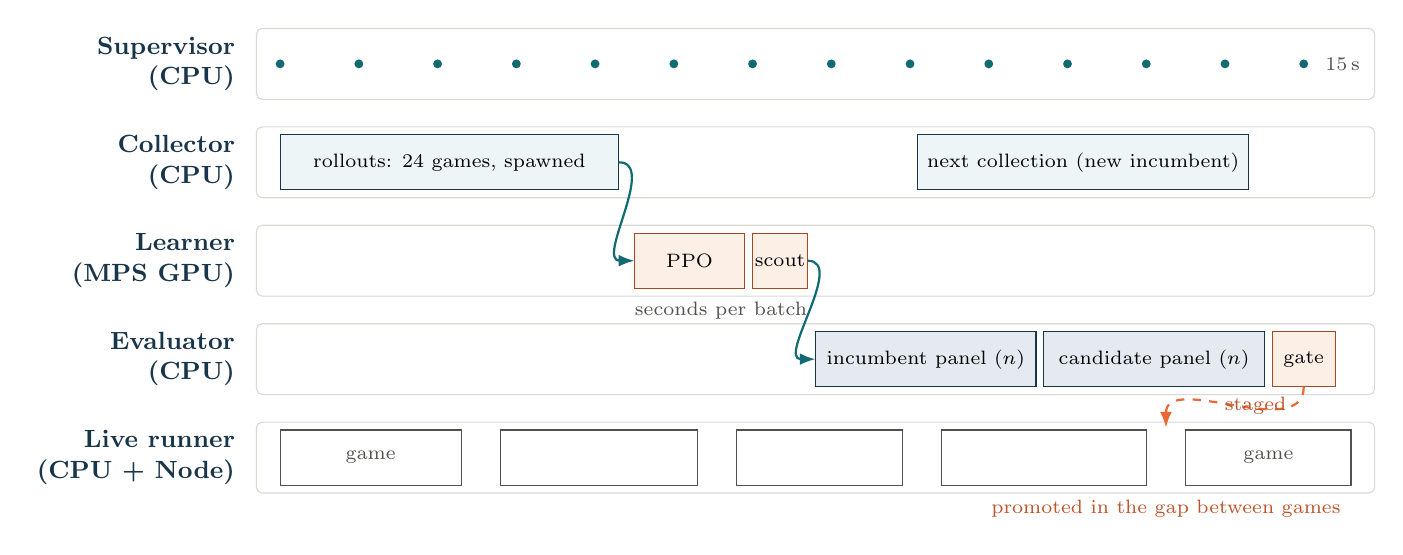
\begin{tikzpicture}[x=1cm,y=1cm]
  \def\W{14.2}
  \foreach \y/\name in {0/{Supervisor\\(CPU)},-1.25/{Collector\\(CPU)},-2.5/{Learner\\(MPS GPU)},-3.75/{Evaluator\\(CPU)},-5.0/{Live runner\\(CPU + Node)}}{
    \draw[lane] (0,\y-0.45) rectangle (\W,\y+0.45);
    \node[lanelabel] at (-0.15,\y) {\name};
  }
  % supervisor ticks
  \foreach \x in {0.3,1.3,...,13.3}{ \fill[accent] (\x,0) circle (1.6pt); }
  \node[note,anchor=west] at (13.45,0) {15\,s};
  % collector
  \fill[pale,draw=ink] (0.3,-1.6) rectangle (4.6,-0.9); \node[font=\scriptsize] at (2.45,-1.25) {rollouts: 24 games, spawned};
  \fill[pale,draw=ink] (8.4,-1.6) rectangle (12.6,-0.9); \node[font=\scriptsize] at (10.5,-1.25) {next collection (new incumbent)};
  % learner
  \fill[warm,draw=seriesB!70!black] (4.8,-2.85) rectangle (6.2,-2.15); \node[font=\scriptsize] at (5.5,-2.5) {PPO};
  \fill[warm,draw=seriesB!70!black] (6.3,-2.85) rectangle (7.0,-2.15); \node[font=\scriptsize] at (6.65,-2.5) {scout};
  \node[note,anchor=north] at (5.9,-2.9) {seconds per batch};
  % evaluator
  \fill[paleink,draw=ink] (7.1,-4.1) rectangle (9.9,-3.4); \node[font=\scriptsize] at (8.5,-3.75) {incumbent panel ($n$)};
  \fill[paleink,draw=ink] (10.0,-4.1) rectangle (12.8,-3.4); \node[font=\scriptsize] at (11.4,-3.75) {candidate panel ($n$)};
  \fill[warm,draw=seriesB!70!black] (12.9,-4.1) rectangle (13.7,-3.4); \node[font=\scriptsize] at (13.3,-3.75) {gate};
  % live runner
  \foreach \a/\b in {0.3/2.6,3.1/5.6,6.1/8.2,8.7/11.3,11.8/13.9}{
    \fill[white,draw=muted] (\a,-5.35) rectangle (\b,-4.65);
  }
  \node[font=\scriptsize,text=muted] at (1.45,-5.0) {game};
  \node[font=\scriptsize,text=muted] at (12.85,-5.0) {game};
  \draw[arr] (4.6,-1.25) to[out=0,in=180] (4.8,-2.5);
  \draw[arr] (7.0,-2.5) to[out=0,in=180] (7.1,-3.75);
  \draw[darr,draw=seriesB] (13.3,-4.1) to[out=-90,in=90] node[note,right,pos=.6,text=seriesB!80!black]{staged} (11.55,-4.62);
  \node[note,text=seriesB!80!black] at (11.55,-5.65) {promoted in the gap between games};
\end{tikzpicture}}
\caption{Schematic timeline of the lanes; durations are not to scale. The
collector and evaluator share one pool of simulator slots. Within the default
budget of four, the evaluator gets half (calibrated locally to three) and the
collector the rest. The learner owns the GPU. The live runner is outside the
pipeline and only ever consumes a staged candidate at a game boundary.}
\label{fig:lanes}
\end{figure}

\subsection{Resource admission}
Every lane re-samples the host before starting work and at minibatch
checkpoints. With $C$ logical cores, a measured CPU load of $u$ percent,
available memory $F$\,GiB, $r$ resident workers and an estimated $m$\,MiB per
worker, the allowed simulator worker count is
\begin{align}
  W_{\mathrm{mem}}&=\max\!\big(0,\lfloor(F-F_{\min})1024/m\rfloor+r\big),\qquad
  W_{\mathrm{cpu}}=\max\!\big(0,\lfloor(u_{\max}-u)C/100\rfloor\big),\\
  W&=\mathbf 1[\text{healthy}]\cdot\max\!\big(0,\min[W_{\max},\,C-C_{\mathrm{res}},\,W_{\mathrm{mem}},\,W_{\mathrm{cpu}}]\big),
\end{align}
where \emph{healthy} means $F\ge F_{\min}$, $u<u_{\max}$, swap-out below its
limit, no critical memory pressure (macOS
\code{kern.memorystatus_vm_pressure_level} flag value~4), and at least 2\,GiB
of free disk. ``Yellow'' pressure (flag value~2) is allowed; only ``red''
blocks. The code
defaults are $C_{\mathrm{res}}=3$, $F_{\min}=2$\,GiB, $W_{\max}=4$,
$u_{\max}=75\%$, $m=400$\,MiB and swap-out 32\,MiB/s. The deployment uses a
modestly higher CPU ceiling and a calibrated swap limit. Optional work also
stops above 90\% of the storage budget (Figure~\ref{fig:storage}).

\begin{proposition}[Headroom invariants]
\label{prop:headroom}
Whenever $W>0$:
\begin{enumerate}
  \item at most $C-C_{\mathrm{res}}$ simulator workers run, so $C_{\mathrm{res}}$
    cores stay free of simulator workers;
  \item if each \emph{new} worker uses at most $m$\,MiB, launching $W-r$ of them
    leaves at least $F_{\min}$ GiB available;
  \item if each worker adds at most $100/C$ percentage points of load (one core),
    the projected load $u+100W/C$ stays at or below $u_{\max}$.
\end{enumerate}
\end{proposition}
\begin{proof}
(1) $W\le C-C_{\mathrm{res}}$. (2) $W-r\le\lfloor(F-F_{\min})1024/m\rfloor$, so
$(W-r)m/1024\le F-F_{\min}$. (3) $W\le\lfloor(u_{\max}-u)C/100\rfloor$ gives
$100W/C\le u_{\max}-u$.
\end{proof}

\intuition{The memory term credits resident workers, whose memory is already
counted in $F$. The CPU term does not credit them, even though their load is
already in $u$. It is therefore conservative and can under-admit while workers
are running. These are cooperative limits enforced by the application, not OS
quotas. Another service can still take the headroom between samples, and the
5-second re-sampling only bounds how long that can go unnoticed.}

\subsection{The MPS lane}
The learner calls
\code{torch.mps.set_per_process_memory_fraction(0.12)}, which caps its Metal
allocations at 12\% of the device's recommended working-set size
\citep{pytorchmps}. Its thread count is limited and it runs at
\code{nice} 10. A GPU duty fraction $d\in(0,1]$ throttles training. After each
optimizer step the learner synchronizes with Metal, measures the step's busy
time $e_k$, and sleeps
\begin{equation}
  s_k=e_k\Big(\frac1d-1\Big).
\end{equation}

\begin{proposition}[Duty cycle]
\label{prop:duty}
Under this rule each step, and therefore any union of steps, has busy fraction
exactly $d$: $\sum_ke_k/\sum_k(e_k+s_k)=d$.
\end{proposition}
\begin{proof}
$e_k+s_k=e_k/d$, so $\sum_k(e_k+s_k)=\sum_ke_k/d$.
\end{proof}
The proposition concerns wall-clock time inside the training loop, measured
after synchronization. It is not a statement about instantaneous GPU
utilization, which the application cannot observe. The default is $d=0.5$.
For these small cached batches, half duty cost several times the full-duty
time: 34.99 vs.\ 7.45\,ms per update in Table~\ref{tab:bench}, which is more
than the factor of two Proposition~\ref{prop:duty} accounts for. The
deployment therefore runs at full duty and relies on the memory cap and the
admission guards (\code{docs/offline-ppo-followup.md}).

\subsection{The tensor cache}
Rebuilding Python feature lists dominated training time, so batches are
converted to tensors once. With $N$ steps and at most $C$ candidates per step,
the resident footprint in float32 is
$N(384\cdot4+C(192\cdot4+1)+8)$ bytes. The extra byte per candidate is its mask
entry and the 8 bytes per step hold the index. The batch is kept on the device
if this is at most $2^{27}$ bytes (128\,MiB). Otherwise a bounded CPU LRU cache
transfers minibatches one at a time.

\begin{example}[When a batch stays resident]
A batch containing a 360-candidate preview has $C=360$, so each step costs
$1536+360\cdot769+8=278{,}384$ bytes. The residency limit is
$\lfloor2^{27}/278{,}384\rfloor=482$ steps. Recent production batches of 404
and 415 steps were resident; a 617-step batch used the CPU cache.
\end{example}

\begin{table}[htbp]
\centering\small
\begin{tabular}{lrr}
\toprule
64-decision batch, up to 360 choices & Before cache (ms/update) & After cache (ms/update) \\
\midrule
CPU & 43.08 & 14.08 \\
MPS, 50\% duty & 121.61 & 34.99 \\
MPS, full duty & 44.06 & 7.45 \\
\bottomrule
\end{tabular}
\caption{Bounded M5 timing windows from \code{docs/m5-learning-orchestration-research.md}.
They were measured while other workloads ran, so they are diagnostic timings
rather than randomized comparisons. A raw kernel benchmark favoured MPS by
only 1.057 vs.\ 1.512\,ms; most of the speedup came from caching.}
\label{tab:bench}
\end{table}

\subsection{Safe reloads of source code}
The \emph{source generation} is a SHA-256 over the entry points,
\code{simulator.cjs}, the lock file and all \code{ml/*.py} files. Rollouts
refuse to run under a mismatched generation. On a change, the supervisor stops
starting children, drains the running ones and exits with code 75 so that
launchd restarts it under the new code. Evaluation plans and staged candidates
record their generation, and promotion refuses a candidate evaluated under
different code. A source change therefore invalidates evaluations; it never
mixes code versions inside one comparison. On 8--9 October, 25 evaluations
were abandoned for this reason and two because the parent had advanced.

\source{\code{ml/pipeline.py} (supervisor, slots), \code{ml/worker.py}
(lanes, collection, learn, evaluate), \code{ml/resources.py}
(\code{ResourcePolicy}, \code{BackgroundGuard}, \code{backend_for}),
\code{ml/batching.py}, \code{ml/reload.py}, \code{ml/simulator.py},
\code{simulator.cjs}, \code{scripts/learning_service.py}.}

\section{Promotion: a paired test and what it can certify}
\label{sec:promotion}

\subsection{The paired design}
For game $i$ the incumbent and the candidate face identical conditions: the
same seed, side, opponent, opponent revision, learner team, opponent team,
open-sheet flag, seed encoding and effective simulator seed. The gate rejects
the run if any of these differ between the two panels. Let
$X_i^I,X_i^C\in\{0,1\}$ be the incumbent's and the candidate's wins in pair
$i$. Pairs with $X_i^I=X_i^C$ are \emph{concordant} and carry no information
about which policy is better. The informative pairs are the gains ($X^C=1$,
$X^I=0$), counted by $g$, and the losses, counted by $\ell$. The discordant
total is $d=g+\ell$, and $W_C-W_I=g-\ell$. Figure~\ref{fig:paired} shows the
idea.

\begin{figure}[htbp]
\centering
\resizebox{\linewidth}{!}{%
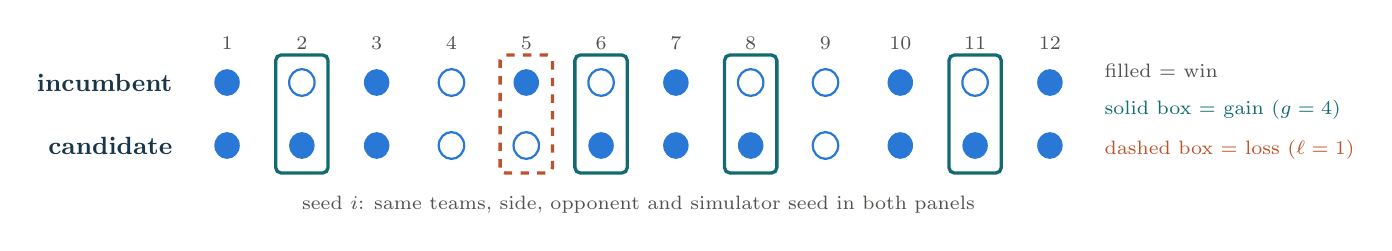
\begin{tikzpicture}[x=0.95cm,y=1cm]
  \foreach \i/\a/\b in {1/1/1,2/0/1,3/1/1,4/0/0,5/1/0,6/0/1,7/1/1,8/0/1,9/0/0,10/1/1,11/0/1,12/1/1}{
    \ifnum\a=1 \fill[seriesA] (\i,0) circle (0.17); \else \draw[seriesA,thick] (\i,0) circle (0.17); \fi
    \ifnum\b=1 \fill[seriesA] (\i,-0.8) circle (0.17); \else \draw[seriesA,thick] (\i,-0.8) circle (0.17); \fi
    \node[note] at (\i,0.5) {\i};
  }
  \foreach \i in {2,6,8,11}{ \draw[draw=accent,very thick,rounded corners=2pt] (\i-0.35,-1.15) rectangle (\i+0.35,0.35); }
  \draw[draw=seriesB!80!black,very thick,rounded corners=2pt,dashed] (5-0.35,-1.15) rectangle (5+0.35,0.35);
  \node[lanelabel] at (0.4,0) {incumbent};
  \node[lanelabel] at (0.4,-0.8) {candidate};
  \node[note,anchor=west] at (12.6,0.15) {filled = win};
  \node[note,anchor=west,text=accent] at (12.6,-0.35) {solid box = gain ($g=4$)};
  \node[note,anchor=west,text=seriesB!80!black] at (12.6,-0.85) {dashed box = loss ($\ell=1$)};
  \node[note] at (6.5,-1.55) {seed $i$: same teams, side, opponent and simulator seed in both panels};
\end{tikzpicture}}
\caption{The paired design on twelve illustrative seeds. Only the five
discordant seeds bear on the comparison. Here $g=4$, $\ell=1$ and
$p=\Prob(\Bin(5,\tfrac12)\ge4)=0.1875$, so this run would fail.}
\label{fig:paired}
\end{figure}

\subsection{The gate}
With $n$ games per policy and margin $m$, a candidate passes when
\begin{equation}
  \text{clean}\ \wedge\ \big(W_C-W_I\ge\lceil nm\rceil\big)\ \wedge\
  p\le0.05,\qquad
  p=\sum_{k=g}^{d}\binom dk2^{-d}\quad(p=1\text{ if }d=0).
  \label{eq:gate}
\end{equation}
\emph{Clean} means: the run is complete and fully paired; there are no
unfinished games and no rejected actions; and every game has a winner or a
tie. The defaults are $n=20$, $m=0.10$; the deployment uses $n=60$, $m=0.05$.
The first edition's gate formula, $\max(1,\lfloor nm+0.999\rfloor)$ with no
test, is obsolete.

\begin{proposition}[Validity of the gate's test]
\label{prop:signtest}
Suppose the pairs are independent, and under the null hypothesis each
discordant pair is equally likely to be a gain or a loss:
$\Prob(X^C=1,X^I=0)=\Prob(X^C=0,X^I=1)$ for every pair. Then
$\Prob(p\le\alpha)\le\alpha$ for every $\alpha\in[0,1]$. In particular, the
gate passes a candidate that is no better than the incumbent with
probability at most 0.05.
\end{proposition}
\begin{proof}
Condition on which pairs are discordant, and hence on $d$. Under the null,
independence and the equal-probability condition make each discordant pair a
gain with probability $\tfrac12$, independently. So $g\mid d\sim\Bin(d,\tfrac12)$.
The statistic $p$ is the upper-tail probability of this exact distribution at
the observed $g$. By the standard property of discrete tail probabilities,
$\Prob(p\le\alpha\mid d)\le\alpha$. Averaging over $d$ preserves the bound.
The other gate conditions only remove passes.
\end{proof}

This is the exact conditional form of McNemar's test \citep{mcnemar}. It needs
neither a normal approximation nor equal marginal rates across pairs. Its
null is ``no systematic difference on the evaluated distribution'', not ``no
difference anywhere''.

\begin{table}[htbp]
\centering\small
\begin{tabular}{rrrr}
\toprule
Discordant pairs $d$ & Minimum gains $g$ & Minimum net $g-\ell$ & $p$ at that $g$ \\
\midrule
4 or fewer & --- & impossible & $\ge0.0625$ \\
5 & 5 & 5 & 0.0313 \\
8 & 7 & 6 & 0.0352 \\
10 & 9 & 8 & 0.0107 \\
15 & 12 & 9 & 0.0176 \\
20 & 15 & 10 & 0.0207 \\
30 & 20 & 10 & 0.0494 \\
40 & 26 & 12 & 0.0403 \\
\bottomrule
\end{tabular}
\caption{What the sign test demands. With $n=60$, $m=0.05$ the margin
requires a net of only $\lceil3\rceil=3$, so the test is always the binding
condition. The one production pass on 9 October was 38 $\to$ 46 wins with
$g=9$, $\ell=1$, $p=0.0107$.}
\label{tab:signtest}
\end{table}

\caveat{The source computes $\lceil nm\rceil$ in floating point. For some
pairs this exceeds the exact ceiling by one; for example
$100\times0.07=7.000000000000001$ rounds up to 8. The configurations actually
used, $(20,0.10)$, $(60,0.05)$, $(96,0.10)$, $(192,0.10)$ and $(200,0.05)$, are
unaffected. A rational or integer form would remove the edge case.}

\subsection{Many gates: multiplicity and the winner's curse}
\label{sec:multiplicity}
One valid test is not the same as a valid campaign of tests. Between 8
October 18:18\,UTC and 9 October 19:57\,UTC the pipeline completed 129 paired
60-game gates, and one passed.

\begin{proposition}[Expected false promotions]
\label{prop:multiplicity}
Run $K$ gates, each with type-I error at most $\alpha$ under its null. If every
candidate is null, the expected number of passes is at most $K\alpha$, and the
probability of at least one pass is at most $\min(1,K\alpha)$. Testing each at
$\alpha/K$ (Bonferroni) bounds the family-wise error by $\alpha$.
\end{proposition}
\begin{proof}
The expected number of passes is the sum of the individual pass probabilities,
each at most $\alpha$ under the null. The union bound gives the second claim
and, with $\alpha/K$, the third.
\end{proof}

With $K=129$ and $\alpha=0.05$, up to 6.45 false passes are possible even if
no candidate is better, so a single pass is not evidence that PPO is improving
the actor. The exact sign test is discrete and conservative, so the true
expectation is somewhat lower, but the conclusion stands. A Bonferroni
threshold would be $0.05/129\approx3.9\times10^{-4}$; the observed $p=0.0107$
does not meet it. The project's own history shows the \emph{winner's curse}
directly. \code{matchup-v1} passed development ($p=0.0068$) and then tied its
independent final 126--126. \code{strategic-v4} reached $p=0.008$ on a
development panel and then went 139--136 on a fresh confirmation ($p=0.39$).
Selection on one panel inflates that panel's apparent effect. An independent,
prospectively specified final panel is the remedy, and the project's
experiment runner (\code{scripts/train_opening.py}) uses one.

\subsection{What the gate does not measure}
Since 9 October the gate evaluates the \emph{sampled self-play actor} against
scripted opponents and a frozen copy of itself. Live turns, however, are
decided by search, and the actor only chooses team previews, greedily. A
candidate that passes therefore improves a decision system that is not the
one deployed for turns. Its effect on live play runs through the preview, and
through the data the next candidates are trained on.
Section~\ref{sec:limits} lists this construct-validity gap as the most
important open problem in the evaluation design.

\subsection{A distribution-free certificate (proposed, not implemented)}
\label{sec:certificate}
A lower confidence bound on the improvement would be a stronger deployment
rule than a test.

\begin{theorem}[Paired Hoeffding lower bound]
\label{thm:evaluation}
Fix both decision systems before evaluation. Draw $n$ evaluation units
independently from a declared target distribution, and in unit $i$ run both
systems on matching conditions. Let $D_i=X_i^C-X_i^I\in[-1,1]$ have common
mean $\Delta$, with $\overline D=n^{-1}\sum_iD_i$. Then, for $\delta\in(0,1)$,
\begin{equation}
  \Prob\!\Big(\Delta\ge\overline D-\sqrt{2\log(1/\delta)/n}\Big)\ge1-\delta.
\label{eq:certificate}
\end{equation}
\end{theorem}
\begin{proof}
Hoeffding's inequality for independent variables in intervals of width 2
gives $\Prob(\overline D-\Delta\ge\eta)\le\exp(-2n^2\eta^2/(4n))=\exp(-n\eta^2/2)$
\citep{hoeffding}. Set $\eta=\sqrt{2\log(1/\delta)/n}$ and take complements.
\end{proof}

\begin{example}[How much evidence a margin is]
At $n=60$ and $\delta=0.05$ the radius is $\sqrt{2\log20/60}\approx0.316$. The
production pass, with $\overline D=8/60\approx0.133$, has lower bound $-0.18$,
so the certificate does not establish improvement. A radius of 0.10 needs
$n\ge\lceil2\log20/0.01\rceil=600$ independent units. The strategic-v1 final,
$\overline D=19/160\approx0.119$ with radius 0.193, is also inconclusive under
this bound, although its exact test gave $p=0.0072$. Hoeffding ignores that
most pairs are concordant. A variance-adaptive or exact
discordant-pair interval is sharper, and is the right next step.
\end{example}

Dependence \emph{within} a pair is allowed; independence \emph{across} units is
required. If both sides of a seed are played, the seed is the unit. If games
cluster by opponent team, the team is the unit: Section~\ref{sec:evidence}
re-tests the search result at that level. For $K$ fixed candidates, use
$\delta/K$ per candidate.

\source{\code{paired_gate}, \code{stage} and \code{promote_ready} in
\code{ml/promotion.py}; \code{evaluate} in \code{ml/worker.py};
preregistered panels in \code{scripts/train_opening.py};
\code{docs/checkpoint-validation.md}.}

\section{Decision-time search}
\label{sec:search}

The learned actor's prior looks one turn ahead against a handful of guessed
opponent moves. The search agent replaces that guess with the official
simulator. It samples complete hypothetical opposing teams, plays every
pairing of our and the opponent's joint actions for one turn, and solves the
resulting matrix game. Figure~\ref{fig:search} shows the procedure.

\begin{figure}[htbp]
\centering
\resizebox{\linewidth}{!}{%
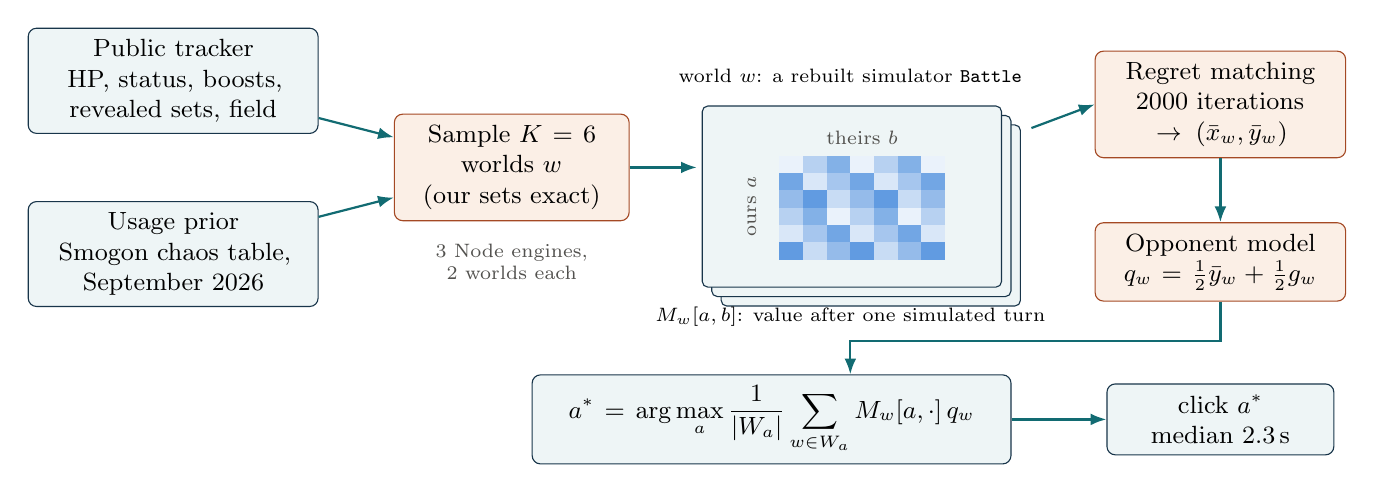
\begin{tikzpicture}[x=1cm,y=1cm]
  \node[box,text width=34mm] (trk) at (0,0) {Public tracker\\HP, status, boosts,\\revealed sets, field};
  \node[box,text width=34mm] (use) at (0,-2.2) {Usage prior\\Smogon chaos table,\\September 2026};
  \node[warmbox,text width=27mm] (smp) at (4.3,-1.1) {Sample $K=6$\\worlds $w$\\(our sets exact)};
  \node[note,anchor=north] at (4.3,-1.95) {3 Node engines,\\2 worlds each};
  \foreach \k in {3,2,1}{
    \draw[draw=ink,fill=pale,rounded corners=2pt] (6.6+0.12*\k,-0.2-0.12*\k) rectangle (10.4+0.12*\k,-2.5-0.12*\k);
  }
  \node[font=\scriptsize,anchor=south] at (8.6,-0.15) {world $w$: a rebuilt simulator \code{Battle}};
  \foreach \i in {0,...,5}{ \foreach \j in {0,...,6}{
     \pgfmathsetmacro{\shade}{mod(7*\i+3*\j,9)*8+10}
     \fill[seriesA!\shade!white] (7.7+0.3*\j,-0.95-0.22*\i) rectangle (8.0+0.3*\j,-1.17-0.22*\i);
  }}
  \node[note] at (8.75,-0.72) {theirs $b$};
  \node[note,rotate=90] at (7.35,-1.6) {ours $a$};
  \node[font=\scriptsize,anchor=north] at (8.6,-2.75) {$M_w[a,b]$: value after one simulated turn};
  \node[warmbox,text width=29mm] (rm) at (13.3,-0.3) {Regret matching\\2000 iterations\\$\to(\bar x_w,\bar y_w)$};
  \node[warmbox,text width=29mm] (bl) at (13.3,-2.3) {Opponent model\\$q_w=\tfrac12\bar y_w+\tfrac12g_w$};
  \node[box,text width=58mm] (avg) at (7.6,-4.3) {$\displaystyle a^*=\arg\max_a\frac1{|W_a|}\sum_{w\in W_a}M_w[a,\cdot]\,q_w$};
  \node[box,text width=26mm] (out) at (13.3,-4.3) {click $a^*$\\median 2.3\,s};
  \draw[arr] (trk) -- (smp); \draw[arr] (use) -- (smp);
  \draw[arr] (smp) -- (6.65,-1.1);
  \draw[arr] (10.9,-0.6) -- (rm.west);
  \draw[arr] (rm) -- (bl);
  \draw[arr] (bl.south) -- ++(0,-0.5) -| ([xshift=10mm]avg.north);
  \draw[arr] (avg) -- (out);
\end{tikzpicture}}
\caption{The search agent. Each world fixes complete hypothetical opposing
sets and copies all public state. Screening keeps at most 24 of our joint
actions and 20 of the opponent's. The payoff matrix of a world therefore needs
at most 480 one-turn simulations, plus up to $4|\B|+4|\A|$ for screening. Team preview is delegated to the learned actor.}
\label{fig:search}
\end{figure}

\subsection{Public tracker}
\code{search/tracker.py} reads only our own player stream. For each
Pok\'{e}mon it tracks:
\begin{itemize}
  \item HP fraction (exact HP when the denominator is not 100), status, sleep
    and toxic counters, boosts and volatiles;
  \item revealed moves, item (or its loss) and ability;
  \item Mega state, last move, and the turn it switched in.
\end{itemize}
For the field it tracks weather, terrain, pseudo-weather and side conditions,
each with its start turn. A condition's remaining duration is estimated as
the base duration minus elapsed turns. If that would be non-positive, the
extended duration is assumed. Open team sheets are parsed from
\code{|showteam|} lines.

\subsection{Sampling hidden sets from usage statistics}
\label{sec:prior}
The prior is Smogon's monthly \emph{chaos} usage table for the format
(September 2026, all ratings, about 1.6 million battles)
\citep{smogonstats}. For each usage entry $e$, which is a species or a Mega
forme, the table gives a raw count $c_e$ and normalized frequencies
$P_e(\cdot)$ that sum to one over each category. The categories are moves,
items, abilities and the 60 most common nature-and-stat-point spreads.

\begin{lemma}[Forme posterior under conditional independence]
\label{lem:forme}
Suppose an opposing Pok\'{e}mon's entry is $e$ with prior probability
proportional to $c_e$. Suppose also that, given $e$, the event ``move $m$ is in
the moveset'' has probability $\pi_e(m)$ independently across moves. Then
after observing the revealed set $R$, $\Prob(e\mid R)\propto
c_e\prod_{m\in R}\pi_e(m)$. If, moreover, $\pi_e(m)=c\,P_e(m)$ for a constant
$c$ shared by all entries (with four move slots, $c\approx4$), then
\begin{equation}
  \Prob(e\mid R)\propto c_e\prod_{m\in R}P_e(m).
  \label{eq:forme}
\end{equation}
\end{lemma}
\begin{proof}
The first statement is Bayes' rule with the likelihood factorized by the
independence assumption. Under the proportionality assumption, the product
becomes $c^{|R|}\prod_{m\in R}P_e(m)$. The factor $c^{|R|}$ is the same for every
entry, so it cancels in the normalization.
\end{proof}

The implementation follows Equation~\eqref{eq:forme}, with three adjustments:
\begin{itemize}
  \item unseen moves get a floor of 0.002 on the share scale, so a surprising
    reveal cannot zero out every entry;
  \item an observed non-stone item, or a spent Mega, removes the Mega entries;
  \item an observed Mega keeps only matching Mega entries.
\end{itemize}
Given $e$, the unrevealed moves are drawn without replacement in proportion
to $P_e$. Item, ability and spread are each drawn from their own marginals. A
Mega entry takes its most common item (assumed to be the stone) and the base
forme's abilities. Unseen previewed Pok\'{e}mon fill the remaining slots,
drawn without replacement in proportion to species usage. When open sheets
were exchanged, species, item, ability, moves and nature are copied exactly,
and only stat points are sampled.

\caveat{Lemma~\ref{lem:forme} is exact only under its independence
assumption. Real movesets have four slots, so move inclusions are negatively
dependent. Item, ability and spread are correlated in real sets, and the
\code{Teammates} table is loaded but unused. The Item Clause is not enforced
across a sampled team. The result is a tractable proposal distribution, not a
calibrated posterior over the opponent's team.}

\subsection{Rebuilding a world}
Each world becomes a fresh simulator \code{Battle} built from both packed
teams. Public state is then written onto it:
\begin{itemize}
  \item formes, abilities, items, exact HP for us and $\mathrm{round}(h\cdot
    \mathrm{maxHP})$ for them, statuses with their counters, and our own PP;
  \item a whitelist of volatiles, such as Protect's stall counter, Substitute,
    Taunt, Encore, Disable and choice lock. The agent does not send last
    moves, so the engine's last-move restoration is unused, and the opponent's
    PP is never set;
  \item weather, terrain and side conditions with their estimated durations.
\end{itemize}
If a side has used its Mega, Mega Evolution is disabled for the whole side.
Our side uses exact sets, HP and PP from our request.

\subsection{The one-turn game in each world}
Our candidates are the Python-legal choices $\A(r)$, pruned in two ways.
Damaging moves at our partner are removed, and when a Mega is available only
Mega-containing choices are kept. Each surviving choice is rewritten by move
\emph{identifier}, because a locked request lists only one move and slot
numbers differ in the rebuilt battle. The opponent's set $\B$ comes from the
engine's own enumeration (Section~\ref{sec:actions}).

\paragraph{Screening.} If $|\B|>20$ or $|\A|>24$, the engine takes four
evenly spaced probe actions $P\subset\A$. It keeps the 20 opponent actions
with the lowest mean value against $P$, which are the best for the opponent.
It then keeps the 24 of our actions with the highest mean value against the
first four kept replies.

\paragraph{Payoffs.} For each remaining pair, the engine restores the world
state, gives the cell its own seed, submits both choices, runs exactly one
turn and evaluates the result:
\begin{equation}
  M_w[a,b]=V\big(\mathrm{Turn}(B_w;a,b;\xi_{w,a,b})\big).
\end{equation}
If the simulator rejects any cell, that cell's whole row (our action) or
column (their action) is removed.

\paragraph{Evaluation function.} A finished battle scores $\pm30$, or 0 for a
tie. Otherwise
$V=S(\text{us})-S(\text{them})+\mathrm{TR}$, where
\begin{equation}
  S=\sum_{\text{alive }p}\big[1+1.2h_p-\mathrm{pen}(p)+\mathbf 1_{\text{active}}\,\beta(p)\big]
   +0.10\cdot\text{Tailwind turns}+0.06\sum\text{screen turns}.
\end{equation}
Status penalties are: paralysis 0.30, freeze 0.50, poison 0.12, toxic 0.25,
sleep $0.45\min(1,\text{turns}/2)$, and burn 0.45 if Attack exceeds Special
Attack, else 0.12. The active-Pok\'{e}mon term $\beta$ rewards offensive,
defensive and speed boosts and a Substitute. It penalizes Perish counts,
confusion, Taunt, Encore, Yawn and Leech Seed. TR is the Trick Room term: it
adds $0.10\cdot\text{turns}\cdot2\clip((\bar v_{\text{them}}-\bar v_{\text{us}})/40,-1,1)$,
where $\bar v$ is each side's mean Speed, so slower teams gain value under Trick Room.

\subsection{Solving the matrix game}
The engine runs simultaneous regret matching on the zero-sum game in which we
maximize $M$ \citep{hartmascolell}. With cumulative regrets $R_t$ for us and
$C_t$ for the opponent,
\begin{align}
  x_t(i)&\propto[R_t(i)]^+,\qquad y_t(j)\propto[C_t(j)]^+\quad(\text{uniform if all}\le0),\\
  R_{t+1}(i)&=R_t(i)+(My_t)_i-x_t^\top My_t,\qquad
  C_{t+1}(j)=C_t(j)+x_t^\top My_t-(x_t^\top M)_j,
\end{align}
for $T=2000$ iterations. It returns the average strategies $\bar x$ and $\bar y$.

\begin{proposition}[Average regret gives an approximate equilibrium]
\label{prop:rm}
Let $\varepsilon_1$ and $\varepsilon_2$ be the two players' average external
regrets after $T$ rounds. Then $(\bar x,\bar y)$ is an
$(\varepsilon_1+\varepsilon_2)$-equilibrium:
$\max_i(M\bar y)_i-\min_j(\bar x^\top M)_j\le\varepsilon_1+\varepsilon_2$.
For regret matching with payoff range $\Delta$,
$\varepsilon_1\le\Delta\sqrt{|\A|/T}$ and $\varepsilon_2\le\Delta\sqrt{|\B|/T}$.
\end{proposition}
\begin{proof}
Let $\bar v=T^{-1}\sum_tx_t^\top My_t$. By linearity,
$T^{-1}\sum_t(My_t)_i=(M\bar y)_i$, so our average regret is
$\max_i(M\bar y)_i-\bar v\le\varepsilon_1$. Likewise the opponent's is
$\bar v-\min_j(\bar x^\top M)_j\le\varepsilon_2$. Adding the two gives the
claim. Because
$\min_j(\bar x^\top M)_j\le\bar x^\top M\bar y\le\max_i(M\bar y)_i$, neither
player can gain more than $\varepsilon_1+\varepsilon_2$ by deviating. The
regret rates are the standard bounds for regret matching
\citep{hartmascolell,zinkevich2007}.
\end{proof}

\intuition{With $|\A|=24$, $|\B|=20$ and $T=2000$, the worst-case gap is
$\Delta(\sqrt{24}+\sqrt{20})/\sqrt{2000}\approx0.21\Delta$. When a terminal
$\pm30$ is reachable, $\Delta$ can be 60, which makes the bound loose. In
practice regret matching usually converges much faster than its worst case.
The bound justifies $\bar y$ only as an approximate equilibrium, and only of
this one-turn surrogate game.}

\subsection{The opponent model and the decision rule}
The agent does \emph{not} play $\bar x$. It treats the opponent as a mixture of
two types:
\begin{equation}
  q_w=\alpha\,\bar y_w+(1-\alpha)\,g_w,\qquad
  g_w(b)\propto\exp\!\big(-(c_b-\min_{b'}c_{b'})/\tau_o\big),\qquad
  c_b=\frac1{|\A|}\sum_aM_w[a,b],
\end{equation}
with $\alpha=\tfrac12$ and $\tau_o=1$. One type plays the equilibrium. The
other is a soft best response to our playing uniformly, a level-1 quantal
response in the sense of \citet{mckelvey1995}. Each world then gives our action
values $U_w(a)=(M_wq_w)_a$. Let $W_a$ be the worlds in which $a$ was valid, and
$W_{\mathrm{ok}}$ the worlds that produced any result. The decision is
\begin{equation}
  a^*=\arg\max_a\Big[\frac1{|W_a|}\sum_{w\in W_a}U_w(a)-0.5\,\mathbf 1\{|W_a|<|W_{\mathrm{ok}}|\}\Big].
  \label{eq:decision}
\end{equation}

\begin{proposition}[Guarantee and exploitability of a best response]
\label{prop:br}
Let $v^*$ be the value of a world's matrix game. For any opponent mixture $y$,
a best response $a^*\in\arg\max_a(My)_a$ satisfies $(My)_{a^*}\ge v^*$. Its
worst case, $\min_bM[a^*,b]$, can still be strictly below $v^*$.
\end{proposition}
\begin{proof}
By the minimax theorem, $v^*=\min_{y'}\max_a(My')_a\le\max_a(My)_a$. For the
second claim take matching pennies, $M=\bigl(\begin{smallmatrix}1&-1\\-1&1\end{smallmatrix}\bigr)$,
with $v^*=0$ and $y=(\tfrac12,\tfrac12)$. Every pure action is a best response,
and each loses 1 to some reply.
\end{proof}

\intuition{Against the \emph{modelled} opponent the pure choice is never worse
than the game's value. Against an opponent who anticipates it, a deterministic
best response can be exploited, whereas $\bar x$ could not be. The design bets
that ladder opponents neither compute this matrix nor exploit its argmax. The
level-1 component also assumes they reason one step about our options. These
are modelling choices, and the live evidence in Section~\ref{sec:evidence} is
too small to test them separately.}

\subsection{Determinization and strategy fusion}
\label{sec:fusion}
Sampling worlds and solving each with full knowledge is \emph{perfect-information
Monte Carlo} (PIMC). It is known to suffer from \emph{strategy fusion}, which
means acting as if one could choose differently in worlds one cannot tell
apart, and from \emph{non-locality} \citep{frankbasin1998}. Yet PIMC often
plays well in practice \citep{long2010}. Information-set search avoids fusion
at a higher cost \citep{cowling2012}. Here the turn decision avoids fusion at
the root: Equation~\eqref{eq:decision} commits to one $a$ for all worlds.
Fusion does enter forced-replacement scoring, which takes
$\frac1K\sum_w\max_aU_w(a)$.

\begin{proposition}[Forced-replacement scores are optimistic]
\label{prop:fusion}
For any values $U_w(a)$,
\[
  \frac1K\sum_w\max_aU_w(a)\ \ge\ \max_a\frac1K\sum_wU_w(a),
\]
with equality if and only if some single action maximizes $U_w$ in every world.
\end{proposition}
\begin{proof}
For each $a'$ and $w$, $\max_aU_w(a)\ge U_w(a')$. Averaging over $w$ and then
maximizing over $a'$ gives the inequality. If $a'$ maximizes in every world,
the two sides coincide. Conversely, if no action does, then for every $a'$
some world has a strict gap, so the average on the left exceeds every
right-hand average.
\end{proof}

\intuition{A replacement whose best follow-up depends on the hidden world is
scored as if we will learn the world before moving. That inflates its value,
so the rule favours flexible-looking replacements whose flexibility is not
real. Within each world both simulated sides also know each other's sets,
even when sheets were not shared, so the opponent model is omniscient about
us.}

\subsection{Monte Carlo error}
Each cell uses one stochastic sample of accuracy, damage rolls and critical
hits. Each cell has its own seed, so two of our actions are not compared under
common random numbers. With $K=6$ worlds, the averaged difference between two
actions has world-sampling noise plus within-cell chance noise.

\begin{proposition}[Ranking two actions]
\label{prop:mc}
Suppose the per-world differences $D_w=U_w(a)-U_w(a')$ are independent, lie in
an interval of width $2\Delta$, and have mean $\gamma>0$. Then the average
over $K$ worlds ranks $a'$ above $a$ with probability at most
$\exp(-K\gamma^2/(2\Delta^2))$.
\end{proposition}
\begin{proof}
This is Hoeffding's inequality applied to the event $\overline D\le0$ with
deviation $\gamma$ \citep{hoeffding}.
\end{proof}

With $K=6$, the bound is useful only when the gap $\gamma$ is a large fraction
of $\Delta$. Small value differences are effectively ranked at random. Common
random numbers across rows, more seeds per cell, or adaptive allocation of
worlds to close decisions would all reduce this noise.

\subsection{Preview, Mega and the learned value}
Team preview is chosen by the actor, greedily. A value-based preview mode
(score 90 plans by the position after preview, averaged over 6 worlds and 3
sampled opposing bring-fours) exists but is untested. Mega Evolution is always
taken when available, for us and for the opponent model, so the agent never
considers saving it. A small value network can replace $V$: 14 features per
Pok\'{e}mon plus field and matchup features, a $128\to128\to1$ ReLU MLP,
trained by binary cross-entropy on omniscient self-play. It blends in as
$(1-\beta)V+\beta\cdot8\tanh(z/2)$, but the deployment uses $\beta=0$, and the
network is neither trained to completion nor gated.

\source{\code{search/agent.py} (worlds, pruning, move-id rewriting, decision
rule, forced replacements), \code{search/engine.cjs} (rebuild, enumeration,
screening, payoffs, regret matching, evaluation), \code{search/priors.py},
\code{search/tracker.py}, \code{search/valuefeat.cjs}, \code{search/train_value.py};
\code{docs/search-agent.md}.}

\section{One live turn: browser transport, guards and viewer}
\label{sec:transport}

\subsection{The sequence}
Figure~\ref{fig:liveturn} follows one turn from the server's request to the
viewer's animation. The browser runner holds an account lock, so only one
controller can drive the account. It reads the official client's state through
\code{app.rooms[id]}, using the request, \code{battle.stepQueue}, the choice
state and the preview order, and acts only by clicking visible controls. It
opens no protocol socket of its own.

\begin{figure}[htbp]
\centering
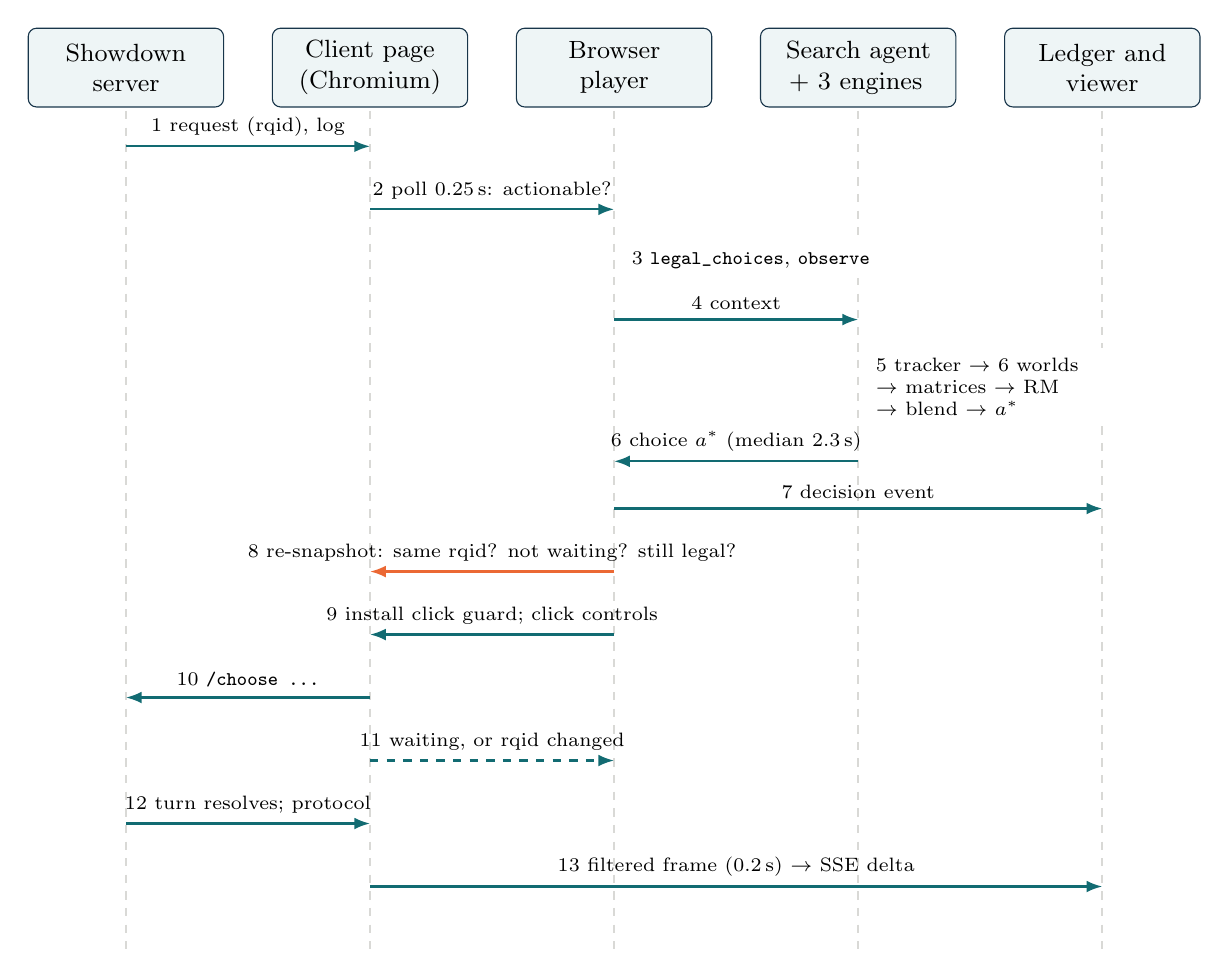
\begin{tikzpicture}[x=1cm,y=1cm]
  \def\H{-11.2}
  \foreach \x/\n in {0/{Showdown\\server},3.1/{Client page\\(Chromium)},6.2/{Browser\\player},9.3/{Search agent\\+ 3 engines},12.4/{Ledger and\\viewer}}{
    \node[box,text width=22mm,minimum height=10mm] at (\x,0) {\n};
    \draw[draw=gridgray,thick,dashed] (\x,-0.55) -- (\x,\H);
  }
  \newcommand{\msg}[5]{\draw[arr,#5] (#1,#3) -- node[font=\scriptsize,above,align=center]{#4} (#2,#3);}
  \msg{0}{3.1}{-1.0}{1 request (rqid), log}{}
  \msg{3.1}{6.2}{-1.8}{2 poll 0.25\,s: actionable?}{}
  \node[font=\scriptsize,align=left,anchor=west,fill=white] at (6.3,-2.45) {3 \code{legal_choices}, \code{observe}};
  \msg{6.2}{9.3}{-3.2}{4 context}{}
  \node[font=\scriptsize,align=left,anchor=west,fill=white,text width=30mm] at (9.4,-4.05) {5 tracker $\to$ 6 worlds\\$\to$ matrices $\to$ RM\\$\to$ blend $\to$ $a^*$};
  \msg{9.3}{6.2}{-5.0}{6 choice $a^*$ (median 2.3\,s)}{}
  \msg{6.2}{12.4}{-5.6}{7 decision event}{}
  \msg{6.2}{3.1}{-6.4}{8 re-snapshot: same rqid? not waiting? still legal?}{draw=seriesB}
  \msg{6.2}{3.1}{-7.2}{9 install click guard; click controls}{}
  \msg{3.1}{0}{-8.0}{10 \code{/choose ...}}{}
  \msg{3.1}{6.2}{-8.8}{11 waiting, or rqid changed}{dashed}
  \msg{0}{3.1}{-9.6}{12 turn resolves; protocol}{}
  \msg{3.1}{12.4}{-10.4}{13 filtered frame (0.2\,s) $\to$ SSE delta}{}
\end{tikzpicture}
\caption{One live turn under search. Step 8 is the freshness check after the
decision. Step 9 installs a capture-phase guard that cancels any click once
the server's rqid has changed. Preview turns replace steps 4--6 with a greedy
actor decision. In recorded mode, steps 4--6 are \code{Brain.decide}.}
\label{fig:liveturn}
\end{figure}

\subsection{Freshness guards}
Search takes seconds and the client keeps animating, so the request on screen
can change while a decision is being computed. Three checks keep a stale
decision from being clicked:
\begin{enumerate}
  \item After deciding, the runner takes a new snapshot. The server rqid must
    be unchanged, the client must not already be waiting, and the choice must
    be legal under the new request. Only the rqid is compared, because the
    client mutates its own copy of the request.
  \item A capture-phase listener on the document cancels any click in the room
    if \code{request.rqid} differs from the guarded rqid, or if the client is
    waiting.
  \item Before each control the runner re-checks the rqid, and it aborts if
    the guard has fired.
\end{enumerate}

\begin{proposition}[Clicks act only on the decided request]
\label{prop:fresh}
Assume that the server assigns a fresh rqid to each request, and that the page
runs JavaScript on a single-threaded event loop. Then every click that
reaches the client's own handler does so while the displayed request has the
rqid the decision was computed for, and while the client is not waiting.
\end{proposition}
\begin{proof}
A click event is dispatched to the capture listener and to the client's
handler within one task of the event loop. A WebSocket message that would
replace the request is processed in a separate task, so it cannot run between
the guard's check and the handler. The guard lets the event proceed only if
the rqid equals the decided one and the client is not waiting. Since rqids are
fresh, equal rqids identify the same request.
\end{proof}

\caveat{The proposition protects individual clicks. A multi-click choice
(Mega checkbox, move, target) can be cut off midway when the request changes,
leaving a partial choice that the next request supersedes. Server acceptance
is confirmed separately, by waiting up to 10\,s for the client to show waiting
or a new rqid. A new \code{|error|}, or an unchanged rqid with a changed
fingerprint, counts as a rejection. At most three submissions are made per
rqid, that is, two retries; a third rejection stops the run.}

\subsection{Recovery}
Two recovery paths exist:
\begin{itemize}
  \item \textbf{Recorded browser runs.} A run that restarts mid-game resubmits
    a saved, unsubmitted proposal only if its stored request equals the
    current one. If the saved proposal was already submitted, the runner stops
    rather than guessing, because the server's acknowledgement is ambiguous.
  \item \textbf{MCP path.} \code{Brain.resume} restores one compatible pending
    episode after a transport failure, with the same identity, steps and
    log-probabilities. It refuses ambiguous fragments or schema changes, and
    resubmits a saved action for the same rqid without resampling, with up to
    three attempts per room.
\end{itemize}
The first edition said that a crash loses the session with no mid-game
reconstruction. That is no longer true, within these limits.

\begin{proposition}[Scope of submission idempotence]
\label{prop:idempotent}
Within one serialized session, a repeated submission for a cached request
sends no second choice unless rejection handling removed the cache entry.
Repeated finalization returns the cached terminal result. A complete stored
episode is never overwritten.
\end{proposition}
\begin{proof}
The choose path checks its cache key before selecting or sending, and finish
returns an existing terminal result first. The store returns early when the
stored identifier is already complete.
\end{proof}
This is not an exactly-once guarantee across processes. A send completing on
the socket is not a server acknowledgement, and an external submission can
still interleave.

\subsection{The live viewer}
The runner publishes filtered public protocol, with names replaced by ``Your
agent'' and ``Opponent'', to an atomically replaced relay file every 0.2\,s.
A small server streams appended lines as server-sent events \citep{sse}. It
sends a full snapshot on a room change or reconnect, and serves only over the
tailnet with HTTPS. The client plays each turn in full. With two or more
turns queued it switches to a faster speed. With four or more it jumps to the
newest turn. A renderer stuck for 15\,s is skipped forward. The viewer is for
observation only and plays no part in decisions.

\source{\code{ml/browser.py} (\code{snapshot}, \code{context}, guards,
\code{submit}, recovery, \code{watch}); \code{scripts/browser_play.py};
\code{scripts/live_watch.py}; \code{web/live-watch/}; \code{ml/live.py}
(\code{resume}, transport recovery); \code{docs/browser-play.md};
\code{docs/live-watch.md}; Playwright \citep{playwright}.}

\section{Opponent-move scouting and team selection}
\label{sec:scout}

\subsection{The public-move scout}
Public logs contain executed events, not private requests or a collecting
policy's probabilities. The repository therefore uses them to train a
classifier, the scout, and never fabricates PPO samples from them.
\code{ingest_public} takes a snapshot of each player's public view at every
turn boundary. A later executed move becomes a label for that snapshot only
if all of the following hold:
\begin{itemize}
  \item the actor was already on the field at the boundary;
  \item the actor is still unambiguous when the move happens;
  \item the move is in the dex;
  \item the move is not tagged \code{[from]} (called or forced).
\end{itemize}
Chat, authentication, HTML and private request lines are removed, and players
are redacted. Incomplete games and orphan samples, whose source battle row is
missing, are excluded.

\begin{proposition}[Turn-boundary non-anticipation]
\label{prop:scout}
If the supplied log is chronological, each retained scout vector is a
function of the prefix up to its turn boundary and of an actor visible in that
prefix. Later moves in the same turn, and later reveals, do not enter it.
\end{proposition}
\begin{proof}
At a \code{turn} event the importer builds the context from the prefix up to
that boundary. When a later move arrives, it encodes the saved context; the
current prefix is used only to reject ambiguous actors. No later prefix is
substituted into a saved context.
\end{proof}
The selection of which examples to keep does use later identity checks. The
proposition is about feature content, not selection independence.

The scout is an MLP: $384\to96$ (tanh) $\to M$. For the live format $M=938$
moves and the network has 127{,}946 parameters. It minimizes
\begin{equation}
  \mathcal L_{\mathrm{scout}}(\psi)=-\frac1N\sum_{n}\log q_\psi(m_n\mid u_n)
\end{equation}
with Adam at learning rate $10^{-3}$, batches of 128, three epochs and
gradient norm 1. Training uses at most 20{,}000 rows. That cap now binds. The
rows used are the 20{,}000 with the smallest hash identifiers, a fixed
pseudo-random tenth of the 192{,}835 M-C samples. A new sample enters training
only if its identifier sorts inside the cap, so the subset behaves like a
uniform subsample that refreshes slowly. Battles whose digest is $0\bmod5$ form the held-out set, so no
battle is split across partitions. A new scout is promoted only with at least
eight held-out samples and no increase in held-out cross-entropy. At inference
the softmax is restricted to the moves on a disclosed sheet, or to the moves
historically seen for the species. The three most likely moves become hashed
state features. Their probabilities are not renormalized, so their sum can be
below one.

\begin{proposition}[Cross-entropy decomposition]
\label{prop:ce}
For a true label distribution $p$ and a prediction $q$ positive on $p$'s
support, $-\sum_mp(m)\log q(m)=H(p)+\KL(p\Vert q)$. The left side is minimized
exactly at $q=p$.
\end{proposition}
\begin{proof}
Add and subtract $\sum_mp\log p$. Then $\KL\ge0$ by Jensen's inequality, with
equality only at $q=p$.
\end{proof}

\caveat{The optimum concerns the distribution of \emph{retained executed}
moves, not opponents' intentions. Inference may also run mid-turn, for example
at a forced replacement, whereas training contexts are taken at turn starts,
so there is a possible distribution shift. Empirically, the scout lowered
held-out cross-entropy, but in a matched battle comparison it changed no
outcomes (0 improved, 0 worsened in 200 games), and recorded-state probes show
the actor responds only weakly to scout features
(\code{docs/offline-ppo-followup.md}).}

\subsection{Team versions as bandit arms}
A team arm is an exact ordered list of sets together with its format. Its
identifier is
\[
  v=\mathrm{SHA256}(\mathrm{canonicalJSON}(\{\mathrm{format},\mathrm{sets}\}))_{1:20},
\]
an 80-bit truncated fingerprint. Canonicalization sorts object keys, not the
party list. Completed outcomes $Y_i$ become scores $z_i=(Y_i+1)/2$, and local
and ladder evidence are queried separately. The posterior uses a
$\mathrm{Beta}(1,1)$ prior:
\begin{equation}
  \alpha_v=1+\sum_iz_i,\quad\beta_v=1+\sum_i(1-z_i),\quad
  \mu_v=\frac{\alpha_v}{\alpha_v+\beta_v},\quad
  \sigma_v^2=\frac{\alpha_v\beta_v}{(\alpha_v+\beta_v)^2(\alpha_v+\beta_v+1)}.
\label{eq:beta}
\end{equation}

\begin{proposition}[Conjugacy, and the tie extension]
\label{prop:beta}
Suppose binary outcomes are conditionally independent and stationary given
$p_v$. Then $w$ wins and $l$ losses update $\mathrm{Beta}(\alpha_0,\beta_0)$ to
$\mathrm{Beta}(\alpha_0+w,\beta_0+l)$. Fractional tie scores follow the same
algebra under the pseudo-likelihood $\prod_ip_v^{z_i}(1-p_v)^{1-z_i}$, which
is not a Bernoulli model of a three-outcome game.
\end{proposition}
\begin{proof}
Multiply the density $\propto p^{\alpha_0-1}(1-p)^{\beta_0-1}$ by
$p^w(1-p)^l$. Replacing the integer counts by score sums gives the same
exponents, but a Bernoulli variable cannot take the value $\tfrac12$.
\end{proof}

\begin{example}[A played and an unplayed team]
Seven wins and three losses give $\mathrm{Beta}(8,4)$, $\mu=2/3$ and
$\sigma=\sqrt{32/1872}\approx0.131$. An unplayed team has $\mu=1/2$ and
$\sigma=\sqrt{1/12}\approx0.289$.
\end{example}

With exploration enabled, the planner draws $\tilde p_v\sim
\mathrm{Beta}(\alpha_v,\beta_v)$ independently and plays
$\arg\max_{v\in C}\tilde p_v$. This is Thompson sampling \citep{thompson}.

\begin{proposition}[Probability matching]
\label{prop:thompson}
Assume independent continuous posteriors over a fixed pool $C$. Then Thompson
sampling selects arm $v$ with probability equal to the posterior probability
that $v$ has the largest \emph{true} success parameter:
$\Prob(\text{select }v)=\Prob_{\text{post}}\big(p_v=\max_{u\in C}p_u\big)$.
\end{proposition}
\begin{proof}
The sampled vector $(\tilde p_u)_{u\in C}$ has the same joint law as the true
parameters $(p_u)_{u\in C}$ under the posterior. The event ``$v$ attains the
maximum'' is therefore equally likely for both vectors. Continuity makes ties
have probability zero.
\end{proof}

\intuition{The first edition stated this with ``largest \emph{sampled}
parameter'', which is circular: the algorithm selects that arm by definition.
The content of the theorem is that sampled and true maxima share one law.}

The estimate describes success \emph{as piloted by the policy of the time,
against the opponents of the time}. It is not intrinsic team quality, and the
posterior is not conditioned on the actor revision. In production the team
was pinned (one candidate, exploration off). Thompson selection was therefore
inactive in the later campaigns, and every live result in
Section~\ref{sec:evidence} uses a single rain team. Variants replace one
member with an attributed same-species set and are validated in the
simulator. Missing stat spreads are generated, labelled as such, and follow
the move categories. A generated Garchomp spread that once boosted the wrong
attacking stat was fixed for this reason.

\source{\code{ingest_public}, \code{public_lines} and \code{Scout} in
\code{ml/scout.py}; \code{rank_teams}, \code{TeamPlanner.plan},
\code{suggest_variants} and \code{generated_spreads} in \code{ml/teams.py};
\code{fingerprint} in \code{ml/storage.py}.}

\section{Evidence}
\label{sec:evidence}

This section collects every quantitative result the project has recorded,
recomputes the exact statistics, and states what each one does and does not
show. Paired tests use the exact one-sided sign test of
Section~\ref{sec:promotion}; all p-values below were recomputed and match the
validation documents. Unless marked otherwise, sources are the repository's
\code{docs/*-validation.md}, \code{docs/opening-policy.md},
\code{docs/post-campaign-learning.md} and \code{docs/search-agent.md}.

\subsection{Paired candidate evaluations}
Figure~\ref{fig:forest} shows the paired experiments on one scale: the
candidate's win rate minus the incumbent's, on the same seeds. Different rows
use different panels, opponents and incumbents, so their totals are not
comparable. Only the direction and the uncertainty of each row are.

\begin{figure}[htbp]
\centering
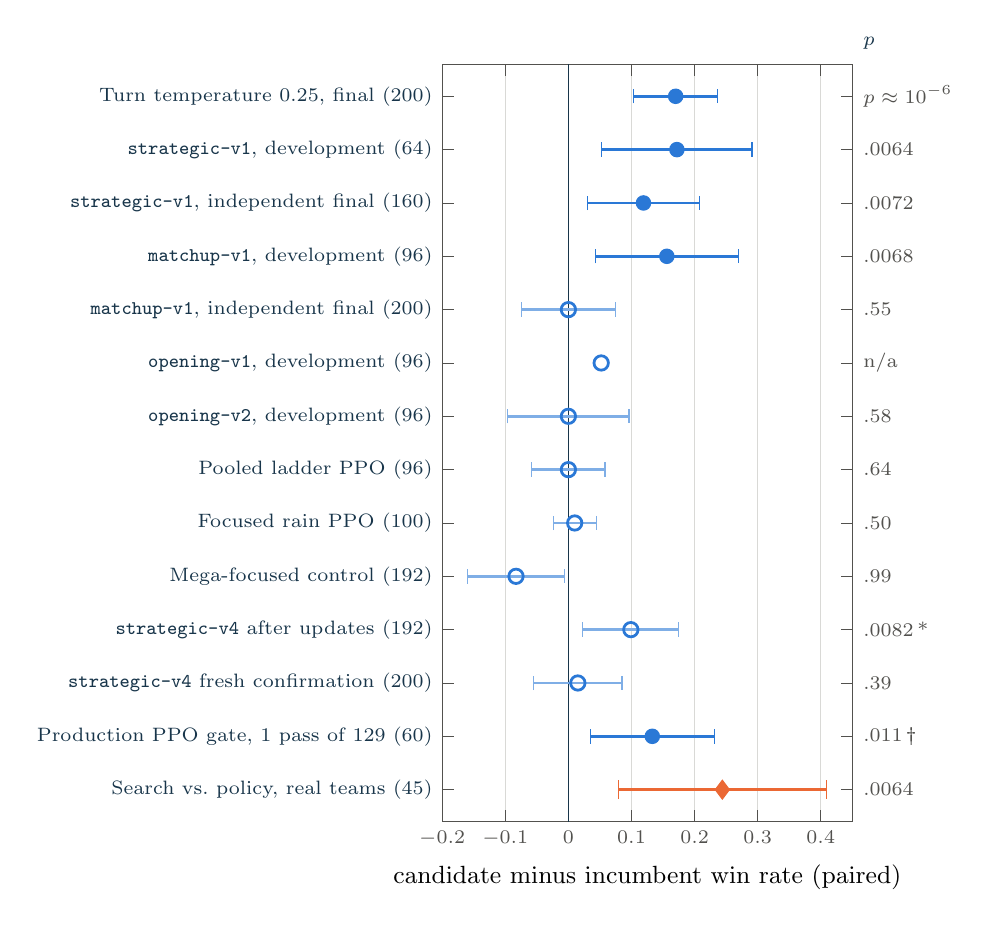
\begin{tikzpicture}
\begin{axis}[
  width=0.56\linewidth, height=11.2cm, scale only axis=false,
  y dir=reverse, ytick={1,...,14}, ymin=0.4, ymax=14.6,
  yticklabels={
    {Turn temperature 0.25, final (200)},
    {\code{strategic-v1}, development (64)},
    {\code{strategic-v1}, independent final (160)},
    {\code{matchup-v1}, development (96)},
    {\code{matchup-v1}, independent final (200)},
    {\code{opening-v1}, development (96)},
    {\code{opening-v2}, development (96)},
    {Pooled ladder PPO (96)},
    {Focused rain PPO (100)},
    {Mega-focused control (192)},
    {\code{strategic-v4} after updates (192)},
    {\code{strategic-v4} fresh confirmation (200)},
    {Production PPO gate, 1 pass of 129 (60)},
    {Search vs.\ policy, real teams (45)}},
  yticklabel style={font=\scriptsize,text=ink},
  xmin=-0.2, xmax=0.45, xtick={-0.2,-0.1,0,0.1,0.2,0.3,0.4},
  xticklabel style={font=\scriptsize,text=muted,/pgf/number format/fixed},
  xlabel={\small candidate minus incumbent win rate (paired)},
  xmajorgrids, grid style={draw=gridgray,thin},
  axis line style={draw=muted}, tick style={draw=muted},
  clip=false]
  \draw[draw=ink,thin] (axis cs:0,0.4) -- (axis cs:0,14.6);
  % passed (filled)
  \addplot[only marks,mark=*,mark size=2.6pt,color=seriesA,
    error bars/.cd,x dir=both,x explicit,error bar style={color=seriesA,line width=1pt}]
    coordinates {(0.170,1) +- (0.067,0) (0.172,2) +- (0.119,0) (0.119,3) +- (0.089,0)
                 (0.156,4) +- (0.113,0) (0.133,13) +- (0.098,0)};
  % failed (hollow)
  \addplot[only marks,mark=o,mark size=2.6pt,color=seriesA,line width=1pt,
    error bars/.cd,x dir=both,x explicit,error bar style={color=seriesA!60,line width=1pt}]
    coordinates {(0.000,5) +- (0.075,0) (0.000,7) +- (0.096,0) (0.000,8) +- (0.058,0)
                 (0.010,9) +- (0.034,0) (-0.083,10) +- (0.077,0) (0.099,11) +- (0.076,0)
                 (0.015,12) +- (0.070,0)};
  \addplot[only marks,mark=o,mark size=2.6pt,color=seriesA,line width=1pt] coordinates {(0.052,6)};
  % search (orange, labelled)
  \addplot[only marks,mark=diamond*,mark size=3.4pt,color=seriesB,
    error bars/.cd,x dir=both,x explicit,error bar style={color=seriesB,line width=1pt}]
    coordinates {(0.244,14) +- (0.165,0)};
  \node[font=\scriptsize,text=muted,anchor=west] at (axis cs:0.452,1) {$p\approx10^{-6}$};
  \node[font=\scriptsize,text=muted,anchor=west] at (axis cs:0.452,2) {.0064};
  \node[font=\scriptsize,text=muted,anchor=west] at (axis cs:0.452,3) {.0072};
  \node[font=\scriptsize,text=muted,anchor=west] at (axis cs:0.452,4) {.0068};
  \node[font=\scriptsize,text=muted,anchor=west] at (axis cs:0.452,5) {.55};
  \node[font=\scriptsize,text=muted,anchor=west] at (axis cs:0.452,6) {n/a};
  \node[font=\scriptsize,text=muted,anchor=west] at (axis cs:0.452,7) {.58};
  \node[font=\scriptsize,text=muted,anchor=west] at (axis cs:0.452,8) {.64};
  \node[font=\scriptsize,text=muted,anchor=west] at (axis cs:0.452,9) {.50};
  \node[font=\scriptsize,text=muted,anchor=west] at (axis cs:0.452,10) {.99};
  \node[font=\scriptsize,text=muted,anchor=west] at (axis cs:0.452,11) {.0082\,*};
  \node[font=\scriptsize,text=muted,anchor=west] at (axis cs:0.452,12) {.39};
  \node[font=\scriptsize,text=muted,anchor=west] at (axis cs:0.452,13) {.011\,\dag};
  \node[font=\scriptsize,text=muted,anchor=west] at (axis cs:0.452,14) {.0064};
  \node[font=\scriptsize\bfseries,text=ink,anchor=west] at (axis cs:0.452,0.0) {$p$};
\end{axis}
\end{tikzpicture}
\caption{Paired evaluations. Filled markers passed their gate and hollow
markers failed. The orange diamond is the search agent, compared with the
learned policy on the same 45 seeds. Bars are approximate 95\% intervals for a
paired difference, $\pm1.96\sqrt{[(g+\ell)/n-((g-\ell)/n)^2]/n}$. The
\code{opening-v1} panel did not report its discordant counts. $^*$ Met $p\le0.05$
but missed the then-required 10-point minimum by one win. $^\dag$ One pass
among 129 gates; see Proposition~\ref{prop:multiplicity}.}
\label{fig:forest}
\end{figure}

Three patterns stand out.
\begin{itemize}
  \item \textbf{Inference-time changes passed; learned weights mostly did not.}
    The large, independently confirmed gains came from the turn temperature
    (same weights, $\tau=0.25$: 95 $\to$ 129 of 200) and from the strategic
    prior (125 vs.\ 106 of 160 on an untouched final). These are changes to
    how the network's scores are used, not to its learned residual.
  \item \textbf{Development wins regress.} \code{matchup-v1} (development
    $p=0.0068$, final tie) and \code{strategic-v4} ($p=0.0082$, then +1.5
    points on fresh seeds) are textbook winner's curses
    (Section~\ref{sec:multiplicity}). Strata of the v4 confirmation show the
    tactical-opponent group \emph{regressing}, from 45 to 38 wins of 55.
  \item \textbf{Search is the largest single effect.} The search agent's paired
    improvement, $+24$ points, is larger than any learned candidate's, with an
    interval that excludes zero.
\end{itemize}

\subsection{The search agent offline}
\begin{table}[htbp]
\centering\small
\begin{tabularx}{\linewidth}{>{\raggedright\arraybackslash}p{0.38\linewidth} X}
\toprule
Test & Result \\
\midrule
Rain mirror, head to head, 40 games, sides alternated & Search 26--14 (65\%);
exact binomial one-sided $p=0.040$. \\
Real teams, paired: same 45 seeds, sides and opponent teams; the
opponent is search-piloted & Policy 19/45 (42\%), search 30/45 (67\%); 14
gains, 3 losses; McNemar one-sided $p=0.0064$ (two-sided 0.013). \\
Same, clustered by opponent team (23 teams, each from both sides, one once) &
13 teams favour search, 2 the policy, 8 tie; sign test $p=0.0037$; exact
sign-flip permutation $p=0.012$. \\
Calibration: policy vs.\ search-piloted real teams & 69/140 (49.3\%), Wilson
95\% [41.1\%, 57.5\%]; close to the live 41\%. \\
Synthetic usage-sampled teams & Policy wins 9--1: \emph{not} a valid proxy for
the ladder. \\
\bottomrule
\end{tabularx}
\caption{Offline search evidence, with open team sheets off. The run ledgers
were recomputed for this report. \code{docs/search-agent.md} describes the
paired panel as ``45 real human teams''; it contains 45 games over 23 distinct
teams. The team-level re-test shows that the effect survives this
clustering.}
\label{tab:searchoffline}
\end{table}

The opponent in the paired test is the search agent itself, piloting teams
that real opponents brought, so the comparison is search against search
versus policy against search. Two incumbent-arm games had a degraded opponent
(12 fallbacks from a forme lookup error, Appendix~\ref{app:defects}). They
were losses in both arms, so they do not change the discordant counts. The
search configuration used for these runs was not recorded in the run files,
which limits exact reproduction.

\subsection{Why raw ladder win rate is not a strength measure}
\label{sec:elo}
Showdown's ladder uses an Elo rating with a floor of 1000 and a rating-dependent
$K$ \citep{showdownladder}. A player of rating $R$ facing $R_o$ has expected
score $E=1/(1+10^{(R_o-R)/400})$ \citep{elo}. A win adds $K_w(1-E)$ and a loss
subtracts $K_\ell E$. Above 1300, $K_w=K_\ell=40$; from 1100 to 1299 both are 50.
At 1000 the winner gains with $K_w=80$ and the loser loses with $K_\ell=20$,
and these interpolate linearly up to 1100.

\begin{proposition}[Stationary win rate under asymmetric $K$]
\label{prop:elo}
Suppose a player keeps a constant true win probability $p$ against opponents
with expected score $E$, so that its expected rating drift is zero. Then
\[
  p=\frac{K_\ell E}{K_w(1-E)+K_\ell E}.
\]
For evenly matched opponents ($E=\tfrac12$), this is $K_\ell/(K_w+K_\ell)$:
0.20 just above the floor, about 0.35 near 1050, and 0.50 from 1100 upward.
The formula assumes no clamp, $R-K_\ell E\ge1000$. At the floor itself a
loss costs nothing, so the stationary $p$ is lower still.
\end{proposition}
\begin{proof}
The expected change is $pK_w(1-E)-(1-p)K_\ell E$. Setting it to zero and
solving for $p$ gives the formula. Substituting $E=\tfrac12$ gives the special
case.
\end{proof}

\intuition{A player who is stable in the 1000--1100 band wins at most 50\%,
and as little as 20\% or less near the floor, simply because of the asymmetric
$K$ and the clamp. The 847-game campaign's
41.1\% is consistent with a policy that hovered in that band. A live goal of
``50\% win rate'' is therefore partly a statement about the rating band. A
steadily rising rating above 1100 is the more informative signal. GXE or a
fixed-rating evaluation pool would be better still.}

\subsection{Live record}
\begin{table}[htbp]
\centering\small
\begin{tabular}{llrr}
\toprule
Games & Decision system & Record & Win rate \\
\midrule
1--100 & Legacy actor; temperature promoted before game 69 & 33--67 & 33\% \\
101--375 & Turn-temperature actor (overnight campaign) & 113--162 & 41\% \\
376--500 & Same actor; corrected rain team & 50--75 & 40\% \\
433--532 & Last 100 before \code{strategic-v1} & 36--64 & 36\% \\
533--632 & \code{strategic-v1}, first 100 & 49--51 & 49\% \\
1--847 & All three generations & 348--499 & 41\% [38, 44] \\
\midrule
41 games, 9 Oct & Search turns; greedy actor preview & 27--14 & 66\% [51, 78] \\
\bottomrule
\end{tabular}
\caption{Live ladder records with Wilson 95\% intervals. These periods are
not randomized comparisons. Team, rating band, opponent pool and transport all
changed between them. The search row counts each battle room once (as of
20:07\,UTC). It includes two losses in which no search decision was submitted,
because of transport or team-validation incidents. Two battles abandoned to
the timer during earlier transport crashes are not in this ledger; counting
them gives 27--16.}
\label{tab:live}
\end{table}

\begin{figure}[htbp]
\centering
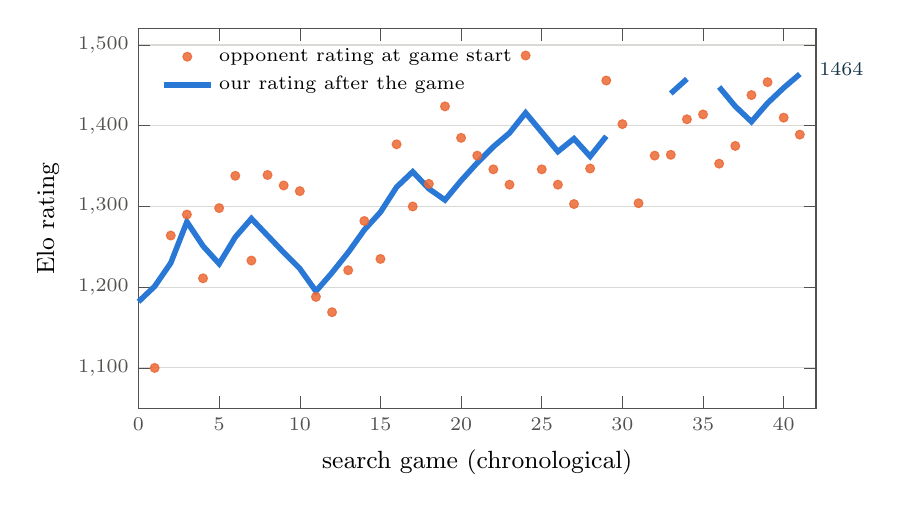
\begin{tikzpicture}
\begin{axis}[
  width=0.84\linewidth, height=6.4cm,
  xmin=0, xmax=42, ymin=1050, ymax=1520,
  xlabel={\small search game (chronological)}, ylabel={\small Elo rating},
  xtick={0,5,...,40}, ytick={1100,1200,1300,1400,1500},
  ticklabel style={font=\scriptsize,text=muted},
  ymajorgrids, grid style={draw=gridgray,thin},
  axis line style={draw=muted}, tick style={draw=muted},
  unbounded coords=jump, legend style={font=\scriptsize,draw=none,fill=none,at={(0.02,0.98)},anchor=north west},
  legend cell align=left, clip=false]
  \addplot[color=seriesB,only marks,mark=*,mark size=1.6pt,opacity=.85] coordinates {
    (1,1100)(2,1264)(3,1290)(4,1211)(5,1298)(6,1338)(7,1233)(8,1339)(9,1326)(10,1319)
    (11,1188)(12,1169)(13,1221)(14,1282)(15,1235)(16,1377)(17,1300)(18,1328)(19,1424)(20,1385)
    (21,1363)(22,1346)(23,1327)(24,1487)(25,1346)(26,1327)(27,1303)(28,1347)(29,1456)(30,1402)
    (31,1304)(32,1363)(33,1364)(34,1408)(35,1414)(36,1353)(37,1375)(38,1438)(39,1454)(40,1410)(41,1389)};
  \addlegendentry{opponent rating at game start}
  \addplot[color=seriesA,line width=2pt,mark=none] coordinates {
    (0,1182)(1,1201)(2,1230)(3,1281)(4,1251)(5,1229)(6,1262)(7,1285)(8,1264)(9,1243)(10,1223)
    (11,1195)(12,1218)(13,1243)(14,1271)(15,1293)(16,1324)(17,1343)(18,1322)(19,1308)(20,1332)
    (21,1354)(22,1374)(23,1391)(24,1416)(25,1392)(26,1368)(27,1384)(28,1362)(29,1387)
    (30,nan)(31,nan)(32,nan)(33,1440)(34,1458)(35,nan)(36,1448)(37,1424)(38,1405)(39,1428)(40,1447)(41,1464)};
  \addlegendentry{our rating after the game}
  \node[font=\scriptsize,text=ink,anchor=west] at (axis cs:41.6,1470) {1464};
\end{axis}
\end{tikzpicture}
\caption{Live rating under the search agent on 9 October 2026. Gaps are games
whose terminal log lacked our rating line. The climb from 1182 to 1464 took
place in the symmetric-$K$ region, where Proposition~\ref{prop:elo} predicts
no drift for a player of stable strength.}
\label{fig:rating}
\end{figure}

\paragraph{Testing the live search record against Elo.} Over the 37 search
games whose logs give both players' pre-game ratings, Elo predicts
$\sum_iE_i=18.4$ wins, with variance $\sum_iE_i(1-E_i)=8.97$. We observed 23 wins,
$z=1.53$. The exact Poisson--binomial upper tail is
$\Prob(X\ge23)=0.086$. Taken alone, the live sample is suggestive but not
significant at 0.05. With the rating climb and the offline paired result, it
is consistent with a real gain. It is \emph{not} an independent confirmation
of the offline effect size. A pre-specified live sample of a few hundred games,
or rating trajectories compared over equal game counts, would settle it.

\subsection{Offline PPO hyperparameter matrix}
Seven settings (learning rate, entropy, collection size, minibatch, epochs and
entropy decay) were trained with three seeds and five updates each. Each was
evaluated against random and tactical opponents, with a sign test, a
conditional bootstrap, and Holm correction over 14 development and 12
final-versus-control hypotheses \citep{holm}. No arm passed after correction.
Two features of the design limit what it shows. The initial heuristic policy
was already strong against random play, and arms with larger collections also
took far fewer optimizer steps, which confounds data size with optimization
exposure. The production hyperparameters were retained
(\code{docs/offline-ppo-followup.md}).

\subsection{Negative results and defects found along the way}
An honest record includes what went wrong. The following were found and
fixed, or are still open, during 7--9 October:
\begin{itemize}
  \item \textbf{Label errors.} Five early wins were stored as losses after an
    identity change (corrected). A coloured public HP string parsed as full HP,
    which is still live in the deployed profile's state encoder
    (Section~\ref{sec:game}). Weather Ball was encoded as a 50-power Normal move
    in rain. A generated Garchomp spread boosted the wrong attacking stat.
  \item \textbf{Design errors.} Simulator seeds were truncated to 16 bits. The
    opponent schedule was confounded with team index. Fourteen orphaned scout
    labels were found. A score cap flattened 288 of 360 preview choices.
    Postgame feedback was silently dropped by the immutable-write rule.
  \item \textbf{Behavioural limits.} Preview entropy was 97.9\% of uniform. The
    preferred four changed in only 4 of 100 cases when the opponent's six
    changed. The pressure curriculum never exercised its intended setup move.
  \item \textbf{Search defects} (Appendix~\ref{app:defects}): a both-Mega
    enumeration drop, a forme lookup failure, unseeded sleep and confusion
    durations, and no common random numbers.
\end{itemize}

\section{Limitations and research directions}
\label{sec:limits}

The system is a working, auditable player with one strong offline result and
a long list of honest failures. Its main open problems follow from the
analysis above, in rough order of importance.

\begin{enumerate}
  \item \textbf{Evaluate the system that is deployed.} The promotion gate
    measures the sampled self-play actor. Live turns are chosen by search.
    A candidate actor should be evaluated as a \emph{preview} policy under
    search turns. Search changes (worlds, opponent blend, evaluation) need a
    gate of their own, with the opponent team as the unit
    (Sections~\ref{sec:promotion} and~\ref{sec:evidence}).
  \item \textbf{Control multiplicity.} The pipeline runs about a hundred gates
    a day. A fixed $\alpha=0.05$ per gate admits several false promotions per
    hundred null candidates. Options are an alpha-spending budget, a
    Bonferroni or Holm level per day, or a mandatory independent final panel,
    which the experiment runner already uses (Proposition~\ref{prop:multiplicity}).
  \item \textbf{Measure strength on a fixed scale.} Live win rate depends on
    the rating band (Proposition~\ref{prop:elo}). Rating trajectories over
    pre-specified game counts, or GXE, should replace raw win rate as the live
    target. A frozen pool of real opponent teams piloted by fixed policies
    should replace synthetic teams as the offline target.
  \item \textbf{Fix the search defects and reduce its noise.} The defects are
    the both-Mega enumeration drop, Mega forcing, forme lookups and unseeded
    durations. Noise can be cut with common random numbers across rows, more
    than one seed per cell, and more worlds for close decisions
    (Proposition~\ref{prop:mc}). The optimistic replacement scoring could be
    replaced by a committed choice across worlds
    (Proposition~\ref{prop:fusion}).
  \item \textbf{Better beliefs.} The usage prior ignores correlations between
    moves, items and spreads, as well as teammates. A joint set model, or a
    posterior updated from damage observations (a revealed roll constrains
    the stat spread), would sharpen the worlds. Information-set search would
    remove fusion at the cost of compute \citep{cowling2012}.
  \item \textbf{State sufficiency.} Fix the legacy HP parser in the deployed
    profile, distinguish unknown from observed values, and test longer
    histories or recurrence. An exact simulator does not help if the encoder
    drops a mechanic.
  \item \textbf{Make learning matter.} Inference-time changes (temperature,
    prior, search) produced every confirmed gain, while gradient updates
    produced almost none. A learned value function for search, trained on
    self-play with the existing value-net pipeline and gated like any
    candidate, is the clearest route by which learning could compound with
    search, in the spirit of \citet{vgcbench}, \citet{metamon} and
    \citet{pokechamp}.
\end{enumerate}

The system has no theorem of equilibrium convergence, optimal team
construction, belief recovery or monotone improvement. Its rigour lies in
stating each implemented contract and each proof assumption explicitly, so
that every new empirical claim can be tested against a defined system.


\appendix
\section{Notation}
\small
\begin{longtable}{p{0.22\linewidth}p{0.71\linewidth}}
\toprule Symbol & Meaning \\
\midrule\endhead
$s_t$, $h_t$ & Latent simulator state; information available before decision $t$. \\
$r$, $\A(r)$ & A Showdown request and its request-visible candidate choices. \\
$x_t$, $z_a$ & State vector in $\R^{384}$; action vector in $\R^{192}$. \\
$q_0$, $f_\theta$, $\ell_\theta$ & Prior (last action coordinate), learned residual, full logit. \\
$\tau$ & Policy temperature; 0.25 for turns and previews in the deployed checkpoint. \\
$\pi_\theta$, $V_\theta$ & Tempered masked policy; critic. \\
$s(a)$, $\kappa$, $g$ & Strategic turn score, pessimism weight, squash $4s/(4+|s|)$. \\
$Y$, $T$, $G_t$ & Terminal outcome, recorded decision count, discounted return. \\
$\gamma$, $\lambda$ & Discount 0.99 and GAE parameter 0.95. \\
$\widehat A_t$, $\widetilde A_t$, $\widehat R_t$ & GAE estimate, standardized advantage, critic target. \\
$\rho_t$, $\epsilon$, $\omega_t$ & Importance ratio, clip width 0.2, phase weight. \\
$\widehat{\KL}$ & Per-epoch estimate $(\rho-1)-\log\rho$; stop threshold 0.03. \\
$W$, $d$ & Admitted simulator workers; GPU duty fraction. \\
$g$, $\ell$, $d$, $p$ & Paired gains, losses, discordant total, exact sign-test p-value
(Section~\ref{sec:promotion}; $d$ also denotes duty in Section~\ref{sec:pipeline}). \\
$n$, $m$ & Games per policy and promotion margin. \\
$w$, $K$, $M_w$ & Sampled world, world count (6 live), per-world payoff matrix. \\
$\bar x_w$, $\bar y_w$, $q_w$ & Regret-matching averages; blended opponent model. \\
$U_w(a)$, $a^*$ & Value of our action in world $w$; chosen action. \\
$E$, $K_w$, $K_\ell$ & Elo expected score; winner and loser $K$ factors. \\
$\psi$, $q_\psi$ & Scout parameters and executed-move distribution. \\
$v$, $\alpha_v$, $\beta_v$, $\mu_v$, $\sigma_v$ & Team version and its Beta posterior summaries. \\
\bottomrule
\end{longtable}
\normalsize

\section{Corrections to the first edition}
\label{app:errata}
\small
\begin{longtable}{>{\raggedright\arraybackslash}p{0.31\linewidth}>{\raggedright\arraybackslash}p{0.62\linewidth}}
\toprule First edition & This edition \\
\midrule\endhead
Snapshot \code{151393d} & A private-history hash absent from the public
repository. This edition cites public \code{0c00ec2}. \\
The actor chooses every live decision & Search chooses turns; the actor
chooses previews greedily (Section~\ref{sec:search}). \\
Policy $\softmax(\ell)$; example $(0.594,0.343,0.063)$ & The policy is
$\softmax(\ell/\tau)$ with $\tau=0.25$. The deployed probabilities for the same
logits are $(0.900,0.100,0.0001)$ (Example~\ref{ex:temperature}). \\
Prior: power$\times$accuracy$\times$STAB$\times$type, zero at preview & This
is the legacy prior. The deployed prior is the squashed scenario score, and it
is nonzero at preview (Section~\ref{sec:strategic}). \\
Preview ordering always matters & Under the strategic profiles the bench is
canonicalized: 360 candidates form 180 plans (Proposition~\ref{prop:preview}). \\
``Not a hypothesis test''; gate $\max(1,\lfloor nm+0.999\rfloor)$ & The gate
is $\lceil nm\rceil$ plus an exact paired sign test at $p\le0.05$
(Equation~\eqref{eq:gate}). \\
The worker promotes, with a 30-minute window & The worker only stages.
Promotion happens before matchmaking, with no pending ladder recording, a
matching parent, hash and source generation. \\
Auxiliary inputs are not frozen & Evaluation freezes content-addressed input
snapshots. \\
No mid-game reconstruction after a crash & Pending-episode resume and
same-rqid resubmission exist (Section~\ref{sec:transport}). \\
Loss: clipped PPO + value + entropy & Now with phase weights, configurable
coefficients, collecting-likelihood exclusion, quality exclusions and an
epoch-level KL stop (Section~\ref{sec:learning}). \\
Consumed ``once produced and evaluated'' & Consumed when the candidate is
saved, before evaluation. \\
Opponents: heuristic plus some random; optional self & The \code{ladder-v1}
cycle (2/8 self, 3/8 tactical, 2/8 heuristic, 1/8 random); 8\% open sheets;
64-bit seeds. \\
Resource rule: load, memory, disk & Adds memory pressure (critical only), the
swap-out rate, the storage budget, and the split between evaluator and
collector. \\
Thompson: ``probability that $v$ has the largest \emph{sampled} parameter'' &
Circular; corrected to the largest \emph{true} parameter
(Proposition~\ref{prop:thompson}). \\
Hashing into $d$ coordinates & Into $d-16$ hashed buckets; 16 are dense
(Proposition~\ref{prop:hash}). \\
Training mask uses a finite minimum & Divided by $\tau<1$, the minimum
overflows to $-\infty$; this is harmless (Section~\ref{sec:network}). \\
``Not a tree search or equilibrium solver'' & True of the network. False of
the deployed system, which solves per-world matrix games. \\
Evidence: two early reports & Section~\ref{sec:evidence}: more than thirty
gates, the search evaluation and the live record. \\
\bottomrule
\end{longtable}
\normalsize

\section{Implementation defects found during this review}
\label{app:defects}
These are reported for transparency. None was changed by this documentation
update.
\begin{enumerate}
  \item \textbf{Both-Mega enumeration drop} (\code{search/engine.cjs},
    \code{sideChoices}). When both actives on a side can Mega Evolve, every move
    option carries \code{ mega}. Each move-and-move pair then has two Mega
    events and is filtered out. Pairs that include a switch survive, so the
    list is not empty and the repair branch never runs; \code{megaFix} is a
    no-op. The side is left with only switch-containing actions. This affects
    opponent worlds in which both sampled actives hold stones, and our own
    forced-replacement look-ahead before our Mega is spent. The fix is to emit
    each move with and without \code{ mega} when \code{canMegaEvo}, and let the
    one-Mega filter choose.
  \item \textbf{Mega always forced.} Delaying Mega Evolution is never
    considered, for us or for the opponent model.
  \item \textbf{Forme lookup.} \code{_our_set} fails for formes whose Mega base
    name differs (for example Floette-Eternal and Floette-Mega). An arena
    opponent fell back 12 times for this reason.
  \item \textbf{Unseeded durations and independent cell seeds.} Rebuilt sleep
    and confusion durations use \code{Math.random}, and each matrix cell has
    its own seed, so rows are not compared under common random numbers.
  \item \textbf{Legacy HP parsing} in the deployed state encoder
    (Section~\ref{sec:game}).
  \item \textbf{Floating-point margin.} $\lceil nm\rceil$ can exceed the exact
    ceiling for some $(n,m)$ (Section~\ref{sec:promotion}).
  \item \textbf{Dead constant.} The burn penalty in the evaluation table is
    overridden by the attack-based rule.
  \item \textbf{Incomplete world state.} Last moves are never sent to the engine,
    so its last-move restoration (and anything that depends on it, such as
    Encore targets) is unused. The opponent's PP is never set.
  \item \textbf{Coarse invalidation.} One rejected matrix cell removes a whole
    row or column of the world's game.
\end{enumerate}

\section{Source-to-claim map}
\label{app:map}
\small
\begin{longtable}{>{\raggedright\arraybackslash}p{0.3\linewidth}p{0.63\linewidth}}
\toprule Source & Claim or object \\
\midrule\endhead
\code{ps_mcp_server.py}, \code{ps_client.py}, \code{harness.py} & 41 MCP
tools; login and transport; team CRUD; legacy loop. \\
\code{battle_state.py} & \code{observe}; \code{legal_choices}; joint
predicates; HP parsers. \\
\code{ml/features.py} & Dimensions 384/192; signed hashing; profiles;
bench canonicalization; prior placement and squash. \\
\code{ml/strategy.py}, \code{ml/tactics.py}, \code{ml/opening.py} & Scenario
hypotheses; deterministic resolution; risk aggregate; damage; preview score. \\
\code{ml/model.py} & 97{,}826-parameter network; temperature; GAE;
likelihood validation; PPO, BC and KL stop; duty cycle. \\
\code{ml/brain.py}, \code{ml/recording.py}, \code{ml/postgame.py} &
Decisions, steps, snapshots, terminal records, resume. \\
\code{ml/data_quality.py} & Trajectory exclusion rules. \\
\code{ml/storage.py}, \code{ml/input_snapshot.py}, \code{ml/data_budget.py} &
Schema, fingerprints, collected checkpoints, frozen inputs, budget. \\
\code{ml/pipeline.py}, \code{ml/worker.py} & Supervisor; lanes; collection
curriculum; learner; evaluator. \\
\code{ml/resources.py}, \code{ml/batching.py}, \code{ml/reload.py} &
Admission and guards; MPS backend; tensor cache; source generation. \\
\code{ml/promotion.py} & Paired gate; sign test; staging; promotion. \\
\code{ml/scout.py}, \code{ml/teams.py}, \code{ml/research.py} & Scout;
Beta/Thompson team choice; research prior. \\
\code{search/agent.py}, \code{search/engine.cjs}, \code{search/priors.py},
\code{search/tracker.py} & Worlds; enumeration; screening; regret matching;
blend; decision; evaluation. \\
\code{ml/browser.py}, \code{scripts/browser_play.py}, \code{scripts/live_watch.py} &
Browser turn; guards; recovery; viewer. \\
\code{simulator.cjs}, \code{ml/simulator.py} & Official simulation and
validation; player streams; local opponents. \\
\code{experiments/}, \code{notebooks/} & Offline PPO matrix and analysis. \\
\bottomrule
\end{longtable}
\normalsize

\section{Reproduction and build}
Build from \code{docs/paper/} with \code{tectonic main.tex} (or
\code{latexmk -pdf main.tex}). The figures are TikZ and pgfplots, with no
external images. To reproduce an experiment, record at least:
\begin{enumerate}
  \item repository and simulator revisions, format, dependency versions,
    feature profile, temperatures, device and seeds;
  \item exact teams with their order and generated-spread flags, learner side,
    opponent policy and revision;
  \item frozen input snapshots, collection mode and terminal, unfinished and
    rejected counts;
  \item for search: worlds, engines, screening sizes, the usage month and
    cutoff, $\alpha$, $\tau_o$, iterations and the seed;
  \item the evaluation unit (game, seed or opponent team), the panel's
    independence from development, and the multiplicity plan.
\end{enumerate}
Use an isolated data root for experiments, because the ordinary root is live
learning state. The offline test suite checks the implemented contracts
(enumeration, masking, collection modes, likelihoods, terminal recording,
reloads, scout non-anticipation, promotion predicates). Passing it is not a
measurement of playing strength.


\begingroup
\small\raggedright
\bibliographystyle{plainnat}
\bibliography{references}
\endgroup
\end{document}
